\documentclass[twoside]{book}

% Packages required by doxygen
\usepackage{calc}
\usepackage{doxygen}
\usepackage{graphicx}
\usepackage[utf8]{inputenc}
\usepackage{makeidx}
\usepackage{multicol}
\usepackage{multirow}
\usepackage{textcomp}
\usepackage[table]{xcolor}

% Font selection
\usepackage[T1]{fontenc}
\usepackage{mathptmx}
\usepackage[scaled=.90]{helvet}
\usepackage{courier}
\usepackage{amssymb}
\usepackage{sectsty}
\renewcommand{\familydefault}{\sfdefault}
\allsectionsfont{%
  \fontseries{bc}\selectfont%
  \color{darkgray}%
}
\renewcommand{\DoxyLabelFont}{%
  \fontseries{bc}\selectfont%
  \color{darkgray}%
}

% Page & text layout
\usepackage{geometry}
\geometry{%
  a4paper,%
  top=2.5cm,%
  bottom=2.5cm,%
  left=2.5cm,%
  right=2.5cm%
}
\tolerance=750
\hfuzz=15pt
\hbadness=750
\setlength{\emergencystretch}{15pt}
\setlength{\parindent}{0cm}
\setlength{\parskip}{0.2cm}
\makeatletter
\renewcommand{\paragraph}{%
  \@startsection{paragraph}{4}{0ex}{-1.0ex}{1.0ex}{%
    \normalfont\normalsize\bfseries\SS@parafont%
  }%
}
\renewcommand{\subparagraph}{%
  \@startsection{subparagraph}{5}{0ex}{-1.0ex}{1.0ex}{%
    \normalfont\normalsize\bfseries\SS@subparafont%
  }%
}
\makeatother

% Headers & footers
\usepackage{fancyhdr}
\pagestyle{fancyplain}
\fancyhead[LE]{\fancyplain{}{\bfseries\thepage}}
\fancyhead[CE]{\fancyplain{}{}}
\fancyhead[RE]{\fancyplain{}{\bfseries\leftmark}}
\fancyhead[LO]{\fancyplain{}{\bfseries\rightmark}}
\fancyhead[CO]{\fancyplain{}{}}
\fancyhead[RO]{\fancyplain{}{\bfseries\thepage}}
\fancyfoot[LE]{\fancyplain{}{}}
\fancyfoot[CE]{\fancyplain{}{}}
\fancyfoot[RE]{\fancyplain{}{\bfseries\scriptsize Generated on Wed Mar 5 2014 12\-:40\-:24 for Programa by Doxygen }}
\fancyfoot[LO]{\fancyplain{}{\bfseries\scriptsize Generated on Wed Mar 5 2014 12\-:40\-:24 for Programa by Doxygen }}
\fancyfoot[CO]{\fancyplain{}{}}
\fancyfoot[RO]{\fancyplain{}{}}
\renewcommand{\footrulewidth}{0.4pt}
\renewcommand{\chaptermark}[1]{%
  \markboth{#1}{}%
}
\renewcommand{\sectionmark}[1]{%
  \markright{\thesection\ #1}%
}

% Indices & bibliography
\usepackage{natbib}
\usepackage[titles]{tocloft}
\setcounter{tocdepth}{3}
\setcounter{secnumdepth}{5}
\makeindex

% Hyperlinks (required, but should be loaded last)
\usepackage{ifpdf}
\ifpdf
  \usepackage[pdftex,pagebackref=true]{hyperref}
\else
  \usepackage[ps2pdf,pagebackref=true]{hyperref}
\fi
\hypersetup{%
  colorlinks=true,%
  linkcolor=blue,%
  citecolor=blue,%
  unicode%
}

% Custom commands
\newcommand{\clearemptydoublepage}{%
  \newpage{\pagestyle{empty}\cleardoublepage}%
}


%===== C O N T E N T S =====

\begin{document}

% Titlepage & ToC
\hypersetup{pageanchor=false}
\pagenumbering{roman}
\begin{titlepage}
\vspace*{7cm}
\begin{center}%
{\Large Programa \\[1ex]\large 1.\-0 }\\
\vspace*{1cm}
{\large Generated by Doxygen 1.8.6}\\
\vspace*{0.5cm}
{\small Wed Mar 5 2014 12:40:24}\\
\end{center}
\end{titlepage}
\clearemptydoublepage
\tableofcontents
\clearemptydoublepage
\pagenumbering{arabic}
\hypersetup{pageanchor=true}

%--- Begin generated contents ---
\chapter{File Index}
\section{File List}
Here is a list of all files with brief descriptions\-:\begin{DoxyCompactList}
\item\contentsline{section}{\hyperlink{main_8cpp}{main.\-cpp} }{\pageref{main_8cpp}}{}
\item\contentsline{section}{\hyperlink{stdafx_8cpp}{stdafx.\-cpp} }{\pageref{stdafx_8cpp}}{}
\item\contentsline{section}{\hyperlink{stdafx_8h}{stdafx.\-h} }{\pageref{stdafx_8h}}{}
\item\contentsline{section}{\hyperlink{targetver_8h}{targetver.\-h} }{\pageref{targetver_8h}}{}
\end{DoxyCompactList}

\chapter{File Documentation}
\hypertarget{main_8cpp}{\section{main.\-cpp File Reference}
\label{main_8cpp}\index{main.\-cpp@{main.\-cpp}}
}
{\ttfamily \#include \char`\"{}stdafx.\-h\char`\"{}}\\*
{\ttfamily \#include $<$iostream$>$}\\*
{\ttfamily \#include $<$cstdlib$>$}\\*
{\ttfamily \#include \char`\"{}opencv2/core/core.\-hpp\char`\"{}}\\*
{\ttfamily \#include \char`\"{}opencv2/flann/miniflann.\-hpp\char`\"{}}\\*
{\ttfamily \#include \char`\"{}opencv2/imgproc/imgproc.\-hpp\char`\"{}}\\*
{\ttfamily \#include \char`\"{}opencv2/photo/photo.\-hpp\char`\"{}}\\*
{\ttfamily \#include \char`\"{}opencv2/video/video.\-hpp\char`\"{}}\\*
{\ttfamily \#include \char`\"{}opencv2/features2d/features2d.\-hpp\char`\"{}}\\*
{\ttfamily \#include \char`\"{}opencv2/objdetect/objdetect.\-hpp\char`\"{}}\\*
{\ttfamily \#include \char`\"{}opencv2/calib3d/calib3d.\-hpp\char`\"{}}\\*
{\ttfamily \#include \char`\"{}opencv2/ml/ml.\-hpp\char`\"{}}\\*
{\ttfamily \#include \char`\"{}opencv2/highgui/highgui.\-hpp\char`\"{}}\\*
{\ttfamily \#include \char`\"{}opencv2/contrib/contrib.\-hpp\char`\"{}}\\*
{\ttfamily \#include \char`\"{}opencv2/core/core\-\_\-c.\-h\char`\"{}}\\*
{\ttfamily \#include \char`\"{}opencv2/highgui/highgui\-\_\-c.\-h\char`\"{}}\\*
{\ttfamily \#include \char`\"{}opencv2/imgproc/imgproc\-\_\-c.\-h\char`\"{}}\\*
Include dependency graph for main.\-cpp\-:
\nopagebreak
\begin{figure}[H]
\begin{center}
\leavevmode
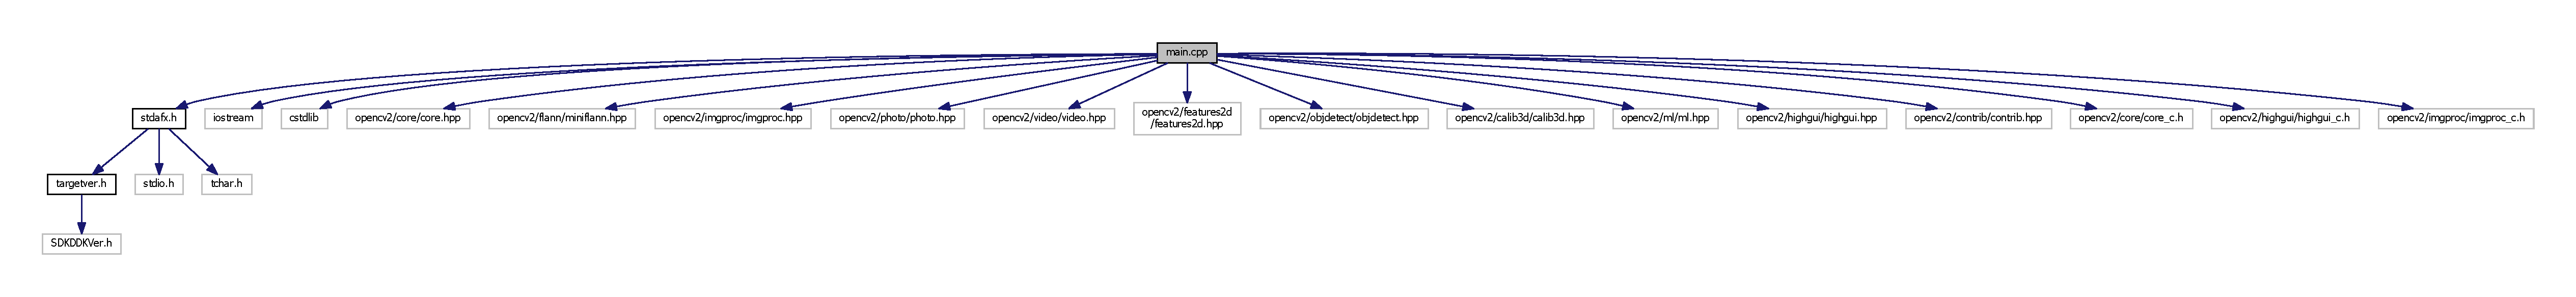
\includegraphics[width=350pt]{main_8cpp__incl}
\end{center}
\end{figure}
\subsection*{Macros}
\begin{DoxyCompactItemize}
\item 
\#define \hyperlink{main_8cpp_a85ea06cb2d8ae7d73119e01073f312d6}{Ax}~11.\-935
\item 
\#define \hyperlink{main_8cpp_ab4c6314e862ec372611b9bc0498394ae}{Bx}~-\/6.\-7718
\item 
\#define \hyperlink{main_8cpp_aa2cb90e056637b106ed2fd71a4e14372}{C\-A\-M\-E\-R\-A\-\_\-\-S\-E\-A\-R\-C\-H}~false
\item 
\#define \hyperlink{main_8cpp_a681e3f587c2e24e577ad99d56b663f0d}{C\-A\-M\-E\-R\-A\-\_\-\-I\-D}~1
\item 
\#define \hyperlink{main_8cpp_ac3b5fd7083022adb2ab1e999c0a8e7d1}{D\-R\-A\-W\-I\-N\-G\-\_\-\-C\-O\-N\-F\-I\-G\-\_\-\-W\-I\-N\-D\-O\-W}~\char`\"{}Referencia -\/ Config\char`\"{}
\item 
\#define \hyperlink{main_8cpp_af2e931be6020e26020a836c1bffc1507}{P\-R\-O\-G\-R\-A\-M\-\_\-\-W\-I\-N\-D\-O\-W}~\char`\"{}Programa\char`\"{}
\item 
\#define \hyperlink{main_8cpp_a2234930167879eb15de58567a2615fa4}{T\-Y\-P\-E\-\_\-\-C\-I\-R\-C\-L\-E}~\char`\"{}C\-I\-R\-C\-L\-E\char`\"{}
\item 
\#define \hyperlink{main_8cpp_a8f71c795785904163fae8bf2510fa686}{T\-Y\-P\-E\-\_\-\-R\-E\-C\-T}~\char`\"{}R\-E\-C\-T\char`\"{}
\item 
\#define \hyperlink{main_8cpp_ae6102eb5288b8f5e0d6ef03190842b1b}{T\-Y\-P\-E\-\_\-\-R\-E\-C\-T2}~\char`\"{}R\-E\-C\-T2\char`\"{}
\item 
\#define \hyperlink{main_8cpp_ad9b4a183f843f4b4c60de13e04624fe9}{M\-A\-X\-\_\-\-D\-R\-A\-W\-I\-N\-G\-\_\-\-C\-I\-R\-C\-L\-E\-\_\-\-R\-A\-D\-I\-U\-S}~400
\item 
\#define \hyperlink{main_8cpp_a0d5912f74422df9b327467244e45f38b}{M\-A\-X\-\_\-\-D\-R\-A\-W\-I\-N\-G\-\_\-\-R\-E\-C\-T\-\_\-\-B\-A\-S\-E}~400
\item 
\#define \hyperlink{main_8cpp_a6d1f72c1dc90c48752f43f4a90fc5902}{M\-A\-X\-\_\-\-D\-R\-A\-W\-I\-N\-G\-\_\-\-R\-E\-C\-T\-\_\-\-H\-E\-I\-G\-H\-T}~400
\item 
\#define \hyperlink{main_8cpp_ac2ac25a24068091b377a725810e748ec}{M\-A\-X\-\_\-\-F\-O\-N\-T\-\_\-\-T\-Y\-P\-E}~7
\item 
\#define \hyperlink{main_8cpp_a24ddddae4a965d15b721a59f224cddbb}{M\-A\-X\-\_\-\-F\-O\-N\-T\-\_\-\-S\-C\-A\-L\-E}~30
\item 
\#define \hyperlink{main_8cpp_a82ffc259b8582be3bd639da25ce880ab}{M\-A\-X\-\_\-\-T\-E\-X\-T\-\_\-\-O\-F\-F\-S\-E\-T}~200
\item 
\#define \hyperlink{main_8cpp_a4e84e5883599bb51a52ecd47374add5f}{M\-A\-X\-\_\-\-L\-E\-F\-T\-\_\-\-T\-E\-X\-T\-\_\-\-O\-F\-F\-S\-E\-T}~50
\item 
\#define \hyperlink{main_8cpp_ac67bb96add6ae84d267d9a8f270a6142}{O\-U\-T\-L\-I\-N\-E\-\_\-\-C\-O\-L\-O\-R}~Scalar(0,255,0)
\item 
\#define \hyperlink{main_8cpp_adde6da43045ef2137942ae981e4f13ca}{O\-U\-T\-L\-I\-N\-E\-\_\-\-T\-H\-I\-C\-K\-N\-E\-S\-S}~4
\item 
\#define \hyperlink{main_8cpp_ab68e4b3d804fc8781d01aca817a71c1e}{T\-E\-X\-T\-\_\-\-T\-H\-I\-C\-K\-N\-E\-S\-S}~3
\item 
\#define \hyperlink{main_8cpp_a9a9b6184443622ad50fd17dbc3d006a6}{F\-U\-L\-L\-\_\-\-W\-H\-E\-I\-G\-H\-T}~1.\-0
\item 
\#define \hyperlink{main_8cpp_a0feaa74b2b5e463d13bd697f8bbd6b24}{T\-H\-R\-E\-E\-\_\-\-F\-O\-U\-R\-T\-H\-S\-\_\-\-W\-H\-E\-I\-G\-H\-T}~0.\-75
\item 
\#define \hyperlink{main_8cpp_a722880a3df1707475b520d9495ed49d5}{H\-A\-L\-F\-\_\-\-W\-H\-E\-I\-G\-H\-T}~0.\-5
\item 
\#define \hyperlink{main_8cpp_aa5e826b79ce951cce04359287eb40b65}{O\-N\-E\-\_\-\-F\-O\-U\-R\-T\-H\-\_\-\-W\-H\-E\-I\-G\-H\-T}~0.\-25
\item 
\#define \hyperlink{main_8cpp_a7c5c9e6093f80f0676571c239290dda1}{N\-O\-\_\-\-W\-H\-E\-I\-G\-H\-T}~0
\item 
\#define \hyperlink{main_8cpp_aa38a7206849a51c5870b8a148bf286af}{sz\-Width}~29
\item 
\#define \hyperlink{main_8cpp_ad815491f23ebc2c71be48b6f215b7937}{sz\-Height}~29
\item 
\#define \hyperlink{main_8cpp_af7cb5eae9c7aa6adb820d43b0652e3da}{delta\-Gaussian\-Blur}~700
\item 
\#define \hyperlink{main_8cpp_a86b6713c598f5468273929392532eade}{min\-Hue}~90
\item 
\#define \hyperlink{main_8cpp_a47c23367137ef58696a7ff35c14a8839}{min\-Sat}~0
\item 
\#define \hyperlink{main_8cpp_a86d9ab7f374e6ea7d65185b705a96628}{min\-Val}~0
\item 
\#define \hyperlink{main_8cpp_af1c86696d8a09abc6e6d123ba2ae19a9}{max\-Hue}~179
\item 
\#define \hyperlink{main_8cpp_acaadb191360d1bbd61de56a372435c83}{max\-Sat}~255
\item 
\#define \hyperlink{main_8cpp_a80484033ea1bd99c5950295c0631cc5b}{max\-Val}~255
\item 
\#define \hyperlink{main_8cpp_a7f59d98329dcda0cc22da8a60dda7d2a}{max\-Points}~10
\item 
\#define \hyperlink{main_8cpp_a1a0e472801c42f908d88f5639d18fc97}{Trans}~80
\item 
\#define \hyperlink{main_8cpp_ace341ba27e87a48423b63d116892319e}{no\-Trans}~100
\item 
\#define \hyperlink{main_8cpp_af4d22e3468e0e9ff30ea4cc4708bf310}{A\-U\-T\-O\-B\-U\-S\-C\-A\-\_\-\-A\-L\-T\-U\-R\-A}~15
\item 
\#define \hyperlink{main_8cpp_a4b664b931e7a93cf91809602933c9313}{A\-U\-T\-O\-B\-U\-S\-C\-A\-\_\-\-L\-A\-R\-G\-U\-R\-A}~5
\item 
\#define \hyperlink{main_8cpp_a2229eef9ff33e056dadf45c70f222814}{P\-R\-E\-C\-I\-S\-A\-O\-\_\-\-B\-U\-S\-C\-A}~1$\ast$\hyperlink{main_8cpp_af4d22e3468e0e9ff30ea4cc4708bf310}{A\-U\-T\-O\-B\-U\-S\-C\-A\-\_\-\-A\-L\-T\-U\-R\-A}$\ast$\hyperlink{main_8cpp_a4b664b931e7a93cf91809602933c9313}{A\-U\-T\-O\-B\-U\-S\-C\-A\-\_\-\-L\-A\-R\-G\-U\-R\-A}
\item 
\#define \hyperlink{main_8cpp_ab996b79d395aa8366c6fafc793c015c4}{M\-I\-N\-I\-M\-A\-L\-\_\-\-M\-A\-T\-C\-H}~0.\-4
\item 
\#define \hyperlink{main_8cpp_a908b1473f4bb5bd5bccb79e90a86554d}{A\-U\-T\-O\-B\-U\-S\-C\-A\-\_\-\-P\-U\-L\-O}~1
\item 
\#define \hyperlink{main_8cpp_aee8c3c363eab49d6a90d3f74587694d5}{A\-P\-P\-R\-O\-X\-I\-M\-A\-T\-I\-O\-N}~3
\item 
\#define \hyperlink{main_8cpp_aa637ca99e2e8b6a736d0910e0f1713bf}{M\-I\-N\-\_\-\-A\-R\-E\-A}~200
\item 
\#define \hyperlink{main_8cpp_a3d4a6aad8b48293253d708f605965036}{M\-A\-X\-\_\-\-A\-R\-E\-A}~400
\item 
\#define \hyperlink{main_8cpp_a2328b6d9f28ba20c7a075084c1e0d30f}{U\-N\-I\-D\-A\-D\-E}~\char`\"{}mg\char`\"{}
\item 
\#define \hyperlink{main_8cpp_a79bcfb6bde984f42d1124b068a509af7}{B\-A\-S\-E}~134
\item 
\#define \hyperlink{main_8cpp_aed89bd71aee8be823e8a20ec4e093c1e}{H\-E\-I\-G\-H\-T}~34
\item 
\#define \hyperlink{main_8cpp_ad173a1378c8a816bb862a618b8adea60}{O\-F\-F\-S\-E\-T\-X}~405
\item 
\#define \hyperlink{main_8cpp_aef854c62d4c998046db3278cce8a12b5}{O\-F\-F\-S\-E\-T\-Y}~356
\item 
\#define \hyperlink{main_8cpp_a105decd3af846926e9dd6edb4fb327b8}{O\-F\-F\-S\-E\-T\-Y\-\_\-2\-R\-E\-C\-T}~50
\item 
\#define \hyperlink{main_8cpp_a6e092cbd5c48e865f9ec561a00cb4475}{E\-R\-R\-\_\-\-N\-O\-\_\-\-C\-A\-M\-E\-R\-A}~-\/32
\item 
\#define \hyperlink{main_8cpp_ae22f9e91229b69c212879a751a75be5f}{E\-R\-R\-\_\-\-L\-O\-A\-D\-\_\-\-C\-A\-M\-E\-R\-A}~-\/33
\item 
\#define \hyperlink{main_8cpp_a9bea9af37686eba317ac82ed8cb24fe3}{E\-R\-R\-\_\-\-I\-N\-I\-T\-I\-A\-L\-\_\-\-R\-E\-A\-D\-\_\-\-F\-R\-A\-M\-E}~-\/34
\item 
\#define \hyperlink{main_8cpp_a9f04ebcfa2cfe642433669071111feec}{E\-R\-R\-\_\-\-R\-E\-A\-D\-\_\-\-F\-R\-A\-M\-E}~-\/35
\item 
\#define \hyperlink{main_8cpp_afde5022330688fc4b60d9d4a0e49372a}{E\-R\-R\-\_\-\-E\-M\-P\-T\-Y\-\_\-\-I\-M\-A\-G\-E\-S}~-\/36
\end{DoxyCompactItemize}
\subsection*{Functions}
\begin{DoxyCompactItemize}
\item 
int \hyperlink{main_8cpp_abf53b5314d2e6e573cda0ab847c4f56a}{search\-Cam} (Video\-Capture $\ast$camera)
\item 
void \hyperlink{main_8cpp_a2c80bf65c83f15c94722f105aa99f9ac}{create\-Draw\-Window} (string name, string \hyperlink{main_8cpp_acce15679d830831b0bbe8ebc2a60b2ca}{type})
\item 
Mat \hyperlink{main_8cpp_aff29bef05524fd9d6b93d005a927e128}{draw\-Model} (string \hyperlink{main_8cpp_acce15679d830831b0bbe8ebc2a60b2ca}{type}, Mat image)
\item 
void \hyperlink{main_8cpp_a34ccd5a5f5e6c89511ed19c070eb3206}{filter} (Mat \&src, Mat \&dst)
\item 
void \hyperlink{main_8cpp_a3cacad06336486e3053a3cd8bdebe09e}{proc} (Mat \&src, Mat \&dst)
\item 
Mat \hyperlink{main_8cpp_a522a59e6315224b9a413b3e06d5bd6ae}{show} (Mat src1, Mat src2, int percentage)
\item 
bool \hyperlink{main_8cpp_a485725f864aa7ae9633b72eb64bcd35d}{all\-Ones} (Mat Vc\-Mat\mbox{[}$\,$\mbox{]}, int Vc\-Size, int num\-Elements)
\item 
void \hyperlink{main_8cpp_adec1dced023c091070e2ea77058e824d}{ajuste} (int Vc\-Size, Range Mat\-Row\mbox{[}$\,$\mbox{]}, Range Mat\-Col\mbox{[}$\,$\mbox{]}, int $\ast$properties\mbox{[}$\,$\mbox{]}, Mat \&src, Mat \&dst)
\item 
vector$<$ vector$<$ Point $>$ $>$ \hyperlink{main_8cpp_ae06205f6d61db52c006bf605c2b2f6f8}{processamento} (Mat H\-S\-V, Mat bin)
\item 
double \hyperlink{main_8cpp_a2eda67e2586d9cd56c494f02239c73e9}{calculation} (vector$<$ vector$<$ Point $>$$>$ region, Mat image)
\item 
int \hyperlink{main_8cpp_a85563ce6e90d50877f86d857c9f57eb9}{\-\_\-tmain} (int argc, char $\ast$$\ast$argv)
\end{DoxyCompactItemize}
\subsection*{Variables}
\begin{DoxyCompactItemize}
\item 
int \hyperlink{main_8cpp_a395279899207ce7f17adf9fdb8ee97ee}{radius}
\item 
int \hyperlink{main_8cpp_a19437a5875428e719515fb20de8a6927}{base}
\item 
int \hyperlink{main_8cpp_ad12fc34ce789bce6c8a05d8a17138534}{height}
\item 
int \hyperlink{main_8cpp_a57abafae3e09830d3569389b2cfcd6d5}{offset\-X}
\item 
int \hyperlink{main_8cpp_ad187214e7b10f8e8d3d271c33dbdb91f}{offset\-Y}
\item 
int \hyperlink{main_8cpp_a76c9a710cb974965ba690749726bdc1d}{text\-\_\-offset\-X}
\item 
int \hyperlink{main_8cpp_ac6035bf74a571f9ad49eefc8823d9537}{text\-\_\-offset\-Y}
\item 
int \hyperlink{main_8cpp_a63d30e1b4d55827d6df4f95076af5d43}{font\-Face}
\item 
int \hyperlink{main_8cpp_a418e7934b5363ecde8269070181b3cef}{scale}
\item 
int \hyperlink{main_8cpp_a86a8ba108d7d4273bf15c0f97f67b7cb}{left\-\_\-text}
\item 
int \hyperlink{main_8cpp_a931521bf226b983dbf1b2c40ee56eec7}{size\-Cols}
\item 
int \hyperlink{main_8cpp_a17cd3d9778d66fe6033661fcdd2d2b63}{size\-Rows}
\item 
string \hyperlink{main_8cpp_acce15679d830831b0bbe8ebc2a60b2ca}{type}
\item 
int \hyperlink{main_8cpp_a45ad72b14f4530cc2c56e634d1b173d7}{\-\_\-sz\-Width}
\item 
int \hyperlink{main_8cpp_a1cc0e1fd2d4da3a678657cd5be953816}{\-\_\-sz\-Height}
\item 
int \hyperlink{main_8cpp_a1dfcb70b9229f2da17dd5922b87ecf2c}{delta}
\item 
int \hyperlink{main_8cpp_a6c156a8f03f7d70255416c642bee7713}{\-\_\-min\-Hue}
\item 
int \hyperlink{main_8cpp_a963e41924775b4d345671ae91326338d}{\-\_\-min\-Sat}
\item 
int \hyperlink{main_8cpp_ae8a1bd1a611103f5cda9e05c9996e0e7}{\-\_\-min\-Val}
\item 
int \hyperlink{main_8cpp_a7f2d59160b6ec5f28816a5c84c2f0387}{\-\_\-max\-Hue}
\item 
int \hyperlink{main_8cpp_a96d19bd8c6abd3ef02e707bad400c96c}{\-\_\-max\-Sat}
\item 
int \hyperlink{main_8cpp_aaa63c2fcee418d0498758ee5f9b28337}{\-\_\-max\-Val}
\end{DoxyCompactItemize}


\subsection{Macro Definition Documentation}
\hypertarget{main_8cpp_aee8c3c363eab49d6a90d3f74587694d5}{\index{main.\-cpp@{main.\-cpp}!A\-P\-P\-R\-O\-X\-I\-M\-A\-T\-I\-O\-N@{A\-P\-P\-R\-O\-X\-I\-M\-A\-T\-I\-O\-N}}
\index{A\-P\-P\-R\-O\-X\-I\-M\-A\-T\-I\-O\-N@{A\-P\-P\-R\-O\-X\-I\-M\-A\-T\-I\-O\-N}!main.cpp@{main.\-cpp}}
\subsubsection[{A\-P\-P\-R\-O\-X\-I\-M\-A\-T\-I\-O\-N}]{\setlength{\rightskip}{0pt plus 5cm}\#define A\-P\-P\-R\-O\-X\-I\-M\-A\-T\-I\-O\-N~3}}\label{main_8cpp_aee8c3c363eab49d6a90d3f74587694d5}


Definition at line 80 of file main.\-cpp.



Referenced by processamento().

\hypertarget{main_8cpp_af4d22e3468e0e9ff30ea4cc4708bf310}{\index{main.\-cpp@{main.\-cpp}!A\-U\-T\-O\-B\-U\-S\-C\-A\-\_\-\-A\-L\-T\-U\-R\-A@{A\-U\-T\-O\-B\-U\-S\-C\-A\-\_\-\-A\-L\-T\-U\-R\-A}}
\index{A\-U\-T\-O\-B\-U\-S\-C\-A\-\_\-\-A\-L\-T\-U\-R\-A@{A\-U\-T\-O\-B\-U\-S\-C\-A\-\_\-\-A\-L\-T\-U\-R\-A}!main.cpp@{main.\-cpp}}
\subsubsection[{A\-U\-T\-O\-B\-U\-S\-C\-A\-\_\-\-A\-L\-T\-U\-R\-A}]{\setlength{\rightskip}{0pt plus 5cm}\#define A\-U\-T\-O\-B\-U\-S\-C\-A\-\_\-\-A\-L\-T\-U\-R\-A~15}}\label{main_8cpp_af4d22e3468e0e9ff30ea4cc4708bf310}


Definition at line 75 of file main.\-cpp.



Referenced by processamento().

\hypertarget{main_8cpp_a4b664b931e7a93cf91809602933c9313}{\index{main.\-cpp@{main.\-cpp}!A\-U\-T\-O\-B\-U\-S\-C\-A\-\_\-\-L\-A\-R\-G\-U\-R\-A@{A\-U\-T\-O\-B\-U\-S\-C\-A\-\_\-\-L\-A\-R\-G\-U\-R\-A}}
\index{A\-U\-T\-O\-B\-U\-S\-C\-A\-\_\-\-L\-A\-R\-G\-U\-R\-A@{A\-U\-T\-O\-B\-U\-S\-C\-A\-\_\-\-L\-A\-R\-G\-U\-R\-A}!main.cpp@{main.\-cpp}}
\subsubsection[{A\-U\-T\-O\-B\-U\-S\-C\-A\-\_\-\-L\-A\-R\-G\-U\-R\-A}]{\setlength{\rightskip}{0pt plus 5cm}\#define A\-U\-T\-O\-B\-U\-S\-C\-A\-\_\-\-L\-A\-R\-G\-U\-R\-A~5}}\label{main_8cpp_a4b664b931e7a93cf91809602933c9313}


Definition at line 76 of file main.\-cpp.



Referenced by processamento().

\hypertarget{main_8cpp_a908b1473f4bb5bd5bccb79e90a86554d}{\index{main.\-cpp@{main.\-cpp}!A\-U\-T\-O\-B\-U\-S\-C\-A\-\_\-\-P\-U\-L\-O@{A\-U\-T\-O\-B\-U\-S\-C\-A\-\_\-\-P\-U\-L\-O}}
\index{A\-U\-T\-O\-B\-U\-S\-C\-A\-\_\-\-P\-U\-L\-O@{A\-U\-T\-O\-B\-U\-S\-C\-A\-\_\-\-P\-U\-L\-O}!main.cpp@{main.\-cpp}}
\subsubsection[{A\-U\-T\-O\-B\-U\-S\-C\-A\-\_\-\-P\-U\-L\-O}]{\setlength{\rightskip}{0pt plus 5cm}\#define A\-U\-T\-O\-B\-U\-S\-C\-A\-\_\-\-P\-U\-L\-O~1}}\label{main_8cpp_a908b1473f4bb5bd5bccb79e90a86554d}


Definition at line 79 of file main.\-cpp.



Referenced by processamento().

\hypertarget{main_8cpp_a85ea06cb2d8ae7d73119e01073f312d6}{\index{main.\-cpp@{main.\-cpp}!Ax@{Ax}}
\index{Ax@{Ax}!main.cpp@{main.\-cpp}}
\subsubsection[{Ax}]{\setlength{\rightskip}{0pt plus 5cm}\#define Ax~11.\-935}}\label{main_8cpp_a85ea06cb2d8ae7d73119e01073f312d6}


Definition at line 39 of file main.\-cpp.



Referenced by \-\_\-tmain().

\hypertarget{main_8cpp_a79bcfb6bde984f42d1124b068a509af7}{\index{main.\-cpp@{main.\-cpp}!B\-A\-S\-E@{B\-A\-S\-E}}
\index{B\-A\-S\-E@{B\-A\-S\-E}!main.cpp@{main.\-cpp}}
\subsubsection[{B\-A\-S\-E}]{\setlength{\rightskip}{0pt plus 5cm}\#define B\-A\-S\-E~134}}\label{main_8cpp_a79bcfb6bde984f42d1124b068a509af7}


Definition at line 84 of file main.\-cpp.



Referenced by \-\_\-tmain().

\hypertarget{main_8cpp_ab4c6314e862ec372611b9bc0498394ae}{\index{main.\-cpp@{main.\-cpp}!Bx@{Bx}}
\index{Bx@{Bx}!main.cpp@{main.\-cpp}}
\subsubsection[{Bx}]{\setlength{\rightskip}{0pt plus 5cm}\#define Bx~-\/6.\-7718}}\label{main_8cpp_ab4c6314e862ec372611b9bc0498394ae}


Definition at line 40 of file main.\-cpp.



Referenced by \-\_\-tmain().

\hypertarget{main_8cpp_a681e3f587c2e24e577ad99d56b663f0d}{\index{main.\-cpp@{main.\-cpp}!C\-A\-M\-E\-R\-A\-\_\-\-I\-D@{C\-A\-M\-E\-R\-A\-\_\-\-I\-D}}
\index{C\-A\-M\-E\-R\-A\-\_\-\-I\-D@{C\-A\-M\-E\-R\-A\-\_\-\-I\-D}!main.cpp@{main.\-cpp}}
\subsubsection[{C\-A\-M\-E\-R\-A\-\_\-\-I\-D}]{\setlength{\rightskip}{0pt plus 5cm}\#define C\-A\-M\-E\-R\-A\-\_\-\-I\-D~1}}\label{main_8cpp_a681e3f587c2e24e577ad99d56b663f0d}


Definition at line 42 of file main.\-cpp.



Referenced by \-\_\-tmain().

\hypertarget{main_8cpp_aa2cb90e056637b106ed2fd71a4e14372}{\index{main.\-cpp@{main.\-cpp}!C\-A\-M\-E\-R\-A\-\_\-\-S\-E\-A\-R\-C\-H@{C\-A\-M\-E\-R\-A\-\_\-\-S\-E\-A\-R\-C\-H}}
\index{C\-A\-M\-E\-R\-A\-\_\-\-S\-E\-A\-R\-C\-H@{C\-A\-M\-E\-R\-A\-\_\-\-S\-E\-A\-R\-C\-H}!main.cpp@{main.\-cpp}}
\subsubsection[{C\-A\-M\-E\-R\-A\-\_\-\-S\-E\-A\-R\-C\-H}]{\setlength{\rightskip}{0pt plus 5cm}\#define C\-A\-M\-E\-R\-A\-\_\-\-S\-E\-A\-R\-C\-H~false}}\label{main_8cpp_aa2cb90e056637b106ed2fd71a4e14372}


Definition at line 41 of file main.\-cpp.



Referenced by \-\_\-tmain().

\hypertarget{main_8cpp_af7cb5eae9c7aa6adb820d43b0652e3da}{\index{main.\-cpp@{main.\-cpp}!delta\-Gaussian\-Blur@{delta\-Gaussian\-Blur}}
\index{delta\-Gaussian\-Blur@{delta\-Gaussian\-Blur}!main.cpp@{main.\-cpp}}
\subsubsection[{delta\-Gaussian\-Blur}]{\setlength{\rightskip}{0pt plus 5cm}\#define delta\-Gaussian\-Blur~700}}\label{main_8cpp_af7cb5eae9c7aa6adb820d43b0652e3da}


Definition at line 65 of file main.\-cpp.



Referenced by \-\_\-tmain().

\hypertarget{main_8cpp_ac3b5fd7083022adb2ab1e999c0a8e7d1}{\index{main.\-cpp@{main.\-cpp}!D\-R\-A\-W\-I\-N\-G\-\_\-\-C\-O\-N\-F\-I\-G\-\_\-\-W\-I\-N\-D\-O\-W@{D\-R\-A\-W\-I\-N\-G\-\_\-\-C\-O\-N\-F\-I\-G\-\_\-\-W\-I\-N\-D\-O\-W}}
\index{D\-R\-A\-W\-I\-N\-G\-\_\-\-C\-O\-N\-F\-I\-G\-\_\-\-W\-I\-N\-D\-O\-W@{D\-R\-A\-W\-I\-N\-G\-\_\-\-C\-O\-N\-F\-I\-G\-\_\-\-W\-I\-N\-D\-O\-W}!main.cpp@{main.\-cpp}}
\subsubsection[{D\-R\-A\-W\-I\-N\-G\-\_\-\-C\-O\-N\-F\-I\-G\-\_\-\-W\-I\-N\-D\-O\-W}]{\setlength{\rightskip}{0pt plus 5cm}\#define D\-R\-A\-W\-I\-N\-G\-\_\-\-C\-O\-N\-F\-I\-G\-\_\-\-W\-I\-N\-D\-O\-W~\char`\"{}Referencia -\/ Config\char`\"{}}}\label{main_8cpp_ac3b5fd7083022adb2ab1e999c0a8e7d1}


Definition at line 43 of file main.\-cpp.



Referenced by \-\_\-tmain().

\hypertarget{main_8cpp_afde5022330688fc4b60d9d4a0e49372a}{\index{main.\-cpp@{main.\-cpp}!E\-R\-R\-\_\-\-E\-M\-P\-T\-Y\-\_\-\-I\-M\-A\-G\-E\-S@{E\-R\-R\-\_\-\-E\-M\-P\-T\-Y\-\_\-\-I\-M\-A\-G\-E\-S}}
\index{E\-R\-R\-\_\-\-E\-M\-P\-T\-Y\-\_\-\-I\-M\-A\-G\-E\-S@{E\-R\-R\-\_\-\-E\-M\-P\-T\-Y\-\_\-\-I\-M\-A\-G\-E\-S}!main.cpp@{main.\-cpp}}
\subsubsection[{E\-R\-R\-\_\-\-E\-M\-P\-T\-Y\-\_\-\-I\-M\-A\-G\-E\-S}]{\setlength{\rightskip}{0pt plus 5cm}\#define E\-R\-R\-\_\-\-E\-M\-P\-T\-Y\-\_\-\-I\-M\-A\-G\-E\-S~-\/36}}\label{main_8cpp_afde5022330688fc4b60d9d4a0e49372a}


Definition at line 97 of file main.\-cpp.



Referenced by \-\_\-tmain().

\hypertarget{main_8cpp_a9bea9af37686eba317ac82ed8cb24fe3}{\index{main.\-cpp@{main.\-cpp}!E\-R\-R\-\_\-\-I\-N\-I\-T\-I\-A\-L\-\_\-\-R\-E\-A\-D\-\_\-\-F\-R\-A\-M\-E@{E\-R\-R\-\_\-\-I\-N\-I\-T\-I\-A\-L\-\_\-\-R\-E\-A\-D\-\_\-\-F\-R\-A\-M\-E}}
\index{E\-R\-R\-\_\-\-I\-N\-I\-T\-I\-A\-L\-\_\-\-R\-E\-A\-D\-\_\-\-F\-R\-A\-M\-E@{E\-R\-R\-\_\-\-I\-N\-I\-T\-I\-A\-L\-\_\-\-R\-E\-A\-D\-\_\-\-F\-R\-A\-M\-E}!main.cpp@{main.\-cpp}}
\subsubsection[{E\-R\-R\-\_\-\-I\-N\-I\-T\-I\-A\-L\-\_\-\-R\-E\-A\-D\-\_\-\-F\-R\-A\-M\-E}]{\setlength{\rightskip}{0pt plus 5cm}\#define E\-R\-R\-\_\-\-I\-N\-I\-T\-I\-A\-L\-\_\-\-R\-E\-A\-D\-\_\-\-F\-R\-A\-M\-E~-\/34}}\label{main_8cpp_a9bea9af37686eba317ac82ed8cb24fe3}


Definition at line 95 of file main.\-cpp.



Referenced by \-\_\-tmain().

\hypertarget{main_8cpp_ae22f9e91229b69c212879a751a75be5f}{\index{main.\-cpp@{main.\-cpp}!E\-R\-R\-\_\-\-L\-O\-A\-D\-\_\-\-C\-A\-M\-E\-R\-A@{E\-R\-R\-\_\-\-L\-O\-A\-D\-\_\-\-C\-A\-M\-E\-R\-A}}
\index{E\-R\-R\-\_\-\-L\-O\-A\-D\-\_\-\-C\-A\-M\-E\-R\-A@{E\-R\-R\-\_\-\-L\-O\-A\-D\-\_\-\-C\-A\-M\-E\-R\-A}!main.cpp@{main.\-cpp}}
\subsubsection[{E\-R\-R\-\_\-\-L\-O\-A\-D\-\_\-\-C\-A\-M\-E\-R\-A}]{\setlength{\rightskip}{0pt plus 5cm}\#define E\-R\-R\-\_\-\-L\-O\-A\-D\-\_\-\-C\-A\-M\-E\-R\-A~-\/33}}\label{main_8cpp_ae22f9e91229b69c212879a751a75be5f}


Definition at line 94 of file main.\-cpp.



Referenced by \-\_\-tmain().

\hypertarget{main_8cpp_a6e092cbd5c48e865f9ec561a00cb4475}{\index{main.\-cpp@{main.\-cpp}!E\-R\-R\-\_\-\-N\-O\-\_\-\-C\-A\-M\-E\-R\-A@{E\-R\-R\-\_\-\-N\-O\-\_\-\-C\-A\-M\-E\-R\-A}}
\index{E\-R\-R\-\_\-\-N\-O\-\_\-\-C\-A\-M\-E\-R\-A@{E\-R\-R\-\_\-\-N\-O\-\_\-\-C\-A\-M\-E\-R\-A}!main.cpp@{main.\-cpp}}
\subsubsection[{E\-R\-R\-\_\-\-N\-O\-\_\-\-C\-A\-M\-E\-R\-A}]{\setlength{\rightskip}{0pt plus 5cm}\#define E\-R\-R\-\_\-\-N\-O\-\_\-\-C\-A\-M\-E\-R\-A~-\/32}}\label{main_8cpp_a6e092cbd5c48e865f9ec561a00cb4475}


Definition at line 93 of file main.\-cpp.



Referenced by search\-Cam().

\hypertarget{main_8cpp_a9f04ebcfa2cfe642433669071111feec}{\index{main.\-cpp@{main.\-cpp}!E\-R\-R\-\_\-\-R\-E\-A\-D\-\_\-\-F\-R\-A\-M\-E@{E\-R\-R\-\_\-\-R\-E\-A\-D\-\_\-\-F\-R\-A\-M\-E}}
\index{E\-R\-R\-\_\-\-R\-E\-A\-D\-\_\-\-F\-R\-A\-M\-E@{E\-R\-R\-\_\-\-R\-E\-A\-D\-\_\-\-F\-R\-A\-M\-E}!main.cpp@{main.\-cpp}}
\subsubsection[{E\-R\-R\-\_\-\-R\-E\-A\-D\-\_\-\-F\-R\-A\-M\-E}]{\setlength{\rightskip}{0pt plus 5cm}\#define E\-R\-R\-\_\-\-R\-E\-A\-D\-\_\-\-F\-R\-A\-M\-E~-\/35}}\label{main_8cpp_a9f04ebcfa2cfe642433669071111feec}


Definition at line 96 of file main.\-cpp.



Referenced by \-\_\-tmain().

\hypertarget{main_8cpp_a9a9b6184443622ad50fd17dbc3d006a6}{\index{main.\-cpp@{main.\-cpp}!F\-U\-L\-L\-\_\-\-W\-H\-E\-I\-G\-H\-T@{F\-U\-L\-L\-\_\-\-W\-H\-E\-I\-G\-H\-T}}
\index{F\-U\-L\-L\-\_\-\-W\-H\-E\-I\-G\-H\-T@{F\-U\-L\-L\-\_\-\-W\-H\-E\-I\-G\-H\-T}!main.cpp@{main.\-cpp}}
\subsubsection[{F\-U\-L\-L\-\_\-\-W\-H\-E\-I\-G\-H\-T}]{\setlength{\rightskip}{0pt plus 5cm}\#define F\-U\-L\-L\-\_\-\-W\-H\-E\-I\-G\-H\-T~1.\-0}}\label{main_8cpp_a9a9b6184443622ad50fd17dbc3d006a6}


Definition at line 58 of file main.\-cpp.



Referenced by draw\-Model().

\hypertarget{main_8cpp_a722880a3df1707475b520d9495ed49d5}{\index{main.\-cpp@{main.\-cpp}!H\-A\-L\-F\-\_\-\-W\-H\-E\-I\-G\-H\-T@{H\-A\-L\-F\-\_\-\-W\-H\-E\-I\-G\-H\-T}}
\index{H\-A\-L\-F\-\_\-\-W\-H\-E\-I\-G\-H\-T@{H\-A\-L\-F\-\_\-\-W\-H\-E\-I\-G\-H\-T}!main.cpp@{main.\-cpp}}
\subsubsection[{H\-A\-L\-F\-\_\-\-W\-H\-E\-I\-G\-H\-T}]{\setlength{\rightskip}{0pt plus 5cm}\#define H\-A\-L\-F\-\_\-\-W\-H\-E\-I\-G\-H\-T~0.\-5}}\label{main_8cpp_a722880a3df1707475b520d9495ed49d5}


Definition at line 60 of file main.\-cpp.

\hypertarget{main_8cpp_aed89bd71aee8be823e8a20ec4e093c1e}{\index{main.\-cpp@{main.\-cpp}!H\-E\-I\-G\-H\-T@{H\-E\-I\-G\-H\-T}}
\index{H\-E\-I\-G\-H\-T@{H\-E\-I\-G\-H\-T}!main.cpp@{main.\-cpp}}
\subsubsection[{H\-E\-I\-G\-H\-T}]{\setlength{\rightskip}{0pt plus 5cm}\#define H\-E\-I\-G\-H\-T~34}}\label{main_8cpp_aed89bd71aee8be823e8a20ec4e093c1e}


Definition at line 85 of file main.\-cpp.



Referenced by \-\_\-tmain().

\hypertarget{main_8cpp_a3d4a6aad8b48293253d708f605965036}{\index{main.\-cpp@{main.\-cpp}!M\-A\-X\-\_\-\-A\-R\-E\-A@{M\-A\-X\-\_\-\-A\-R\-E\-A}}
\index{M\-A\-X\-\_\-\-A\-R\-E\-A@{M\-A\-X\-\_\-\-A\-R\-E\-A}!main.cpp@{main.\-cpp}}
\subsubsection[{M\-A\-X\-\_\-\-A\-R\-E\-A}]{\setlength{\rightskip}{0pt plus 5cm}\#define M\-A\-X\-\_\-\-A\-R\-E\-A~400}}\label{main_8cpp_a3d4a6aad8b48293253d708f605965036}


Definition at line 82 of file main.\-cpp.



Referenced by processamento().

\hypertarget{main_8cpp_ad9b4a183f843f4b4c60de13e04624fe9}{\index{main.\-cpp@{main.\-cpp}!M\-A\-X\-\_\-\-D\-R\-A\-W\-I\-N\-G\-\_\-\-C\-I\-R\-C\-L\-E\-\_\-\-R\-A\-D\-I\-U\-S@{M\-A\-X\-\_\-\-D\-R\-A\-W\-I\-N\-G\-\_\-\-C\-I\-R\-C\-L\-E\-\_\-\-R\-A\-D\-I\-U\-S}}
\index{M\-A\-X\-\_\-\-D\-R\-A\-W\-I\-N\-G\-\_\-\-C\-I\-R\-C\-L\-E\-\_\-\-R\-A\-D\-I\-U\-S@{M\-A\-X\-\_\-\-D\-R\-A\-W\-I\-N\-G\-\_\-\-C\-I\-R\-C\-L\-E\-\_\-\-R\-A\-D\-I\-U\-S}!main.cpp@{main.\-cpp}}
\subsubsection[{M\-A\-X\-\_\-\-D\-R\-A\-W\-I\-N\-G\-\_\-\-C\-I\-R\-C\-L\-E\-\_\-\-R\-A\-D\-I\-U\-S}]{\setlength{\rightskip}{0pt plus 5cm}\#define M\-A\-X\-\_\-\-D\-R\-A\-W\-I\-N\-G\-\_\-\-C\-I\-R\-C\-L\-E\-\_\-\-R\-A\-D\-I\-U\-S~400}}\label{main_8cpp_ad9b4a183f843f4b4c60de13e04624fe9}


Definition at line 48 of file main.\-cpp.



Referenced by create\-Draw\-Window().

\hypertarget{main_8cpp_a0d5912f74422df9b327467244e45f38b}{\index{main.\-cpp@{main.\-cpp}!M\-A\-X\-\_\-\-D\-R\-A\-W\-I\-N\-G\-\_\-\-R\-E\-C\-T\-\_\-\-B\-A\-S\-E@{M\-A\-X\-\_\-\-D\-R\-A\-W\-I\-N\-G\-\_\-\-R\-E\-C\-T\-\_\-\-B\-A\-S\-E}}
\index{M\-A\-X\-\_\-\-D\-R\-A\-W\-I\-N\-G\-\_\-\-R\-E\-C\-T\-\_\-\-B\-A\-S\-E@{M\-A\-X\-\_\-\-D\-R\-A\-W\-I\-N\-G\-\_\-\-R\-E\-C\-T\-\_\-\-B\-A\-S\-E}!main.cpp@{main.\-cpp}}
\subsubsection[{M\-A\-X\-\_\-\-D\-R\-A\-W\-I\-N\-G\-\_\-\-R\-E\-C\-T\-\_\-\-B\-A\-S\-E}]{\setlength{\rightskip}{0pt plus 5cm}\#define M\-A\-X\-\_\-\-D\-R\-A\-W\-I\-N\-G\-\_\-\-R\-E\-C\-T\-\_\-\-B\-A\-S\-E~400}}\label{main_8cpp_a0d5912f74422df9b327467244e45f38b}


Definition at line 49 of file main.\-cpp.



Referenced by create\-Draw\-Window().

\hypertarget{main_8cpp_a6d1f72c1dc90c48752f43f4a90fc5902}{\index{main.\-cpp@{main.\-cpp}!M\-A\-X\-\_\-\-D\-R\-A\-W\-I\-N\-G\-\_\-\-R\-E\-C\-T\-\_\-\-H\-E\-I\-G\-H\-T@{M\-A\-X\-\_\-\-D\-R\-A\-W\-I\-N\-G\-\_\-\-R\-E\-C\-T\-\_\-\-H\-E\-I\-G\-H\-T}}
\index{M\-A\-X\-\_\-\-D\-R\-A\-W\-I\-N\-G\-\_\-\-R\-E\-C\-T\-\_\-\-H\-E\-I\-G\-H\-T@{M\-A\-X\-\_\-\-D\-R\-A\-W\-I\-N\-G\-\_\-\-R\-E\-C\-T\-\_\-\-H\-E\-I\-G\-H\-T}!main.cpp@{main.\-cpp}}
\subsubsection[{M\-A\-X\-\_\-\-D\-R\-A\-W\-I\-N\-G\-\_\-\-R\-E\-C\-T\-\_\-\-H\-E\-I\-G\-H\-T}]{\setlength{\rightskip}{0pt plus 5cm}\#define M\-A\-X\-\_\-\-D\-R\-A\-W\-I\-N\-G\-\_\-\-R\-E\-C\-T\-\_\-\-H\-E\-I\-G\-H\-T~400}}\label{main_8cpp_a6d1f72c1dc90c48752f43f4a90fc5902}


Definition at line 50 of file main.\-cpp.



Referenced by create\-Draw\-Window().

\hypertarget{main_8cpp_a24ddddae4a965d15b721a59f224cddbb}{\index{main.\-cpp@{main.\-cpp}!M\-A\-X\-\_\-\-F\-O\-N\-T\-\_\-\-S\-C\-A\-L\-E@{M\-A\-X\-\_\-\-F\-O\-N\-T\-\_\-\-S\-C\-A\-L\-E}}
\index{M\-A\-X\-\_\-\-F\-O\-N\-T\-\_\-\-S\-C\-A\-L\-E@{M\-A\-X\-\_\-\-F\-O\-N\-T\-\_\-\-S\-C\-A\-L\-E}!main.cpp@{main.\-cpp}}
\subsubsection[{M\-A\-X\-\_\-\-F\-O\-N\-T\-\_\-\-S\-C\-A\-L\-E}]{\setlength{\rightskip}{0pt plus 5cm}\#define M\-A\-X\-\_\-\-F\-O\-N\-T\-\_\-\-S\-C\-A\-L\-E~30}}\label{main_8cpp_a24ddddae4a965d15b721a59f224cddbb}


Definition at line 52 of file main.\-cpp.



Referenced by create\-Draw\-Window().

\hypertarget{main_8cpp_ac2ac25a24068091b377a725810e748ec}{\index{main.\-cpp@{main.\-cpp}!M\-A\-X\-\_\-\-F\-O\-N\-T\-\_\-\-T\-Y\-P\-E@{M\-A\-X\-\_\-\-F\-O\-N\-T\-\_\-\-T\-Y\-P\-E}}
\index{M\-A\-X\-\_\-\-F\-O\-N\-T\-\_\-\-T\-Y\-P\-E@{M\-A\-X\-\_\-\-F\-O\-N\-T\-\_\-\-T\-Y\-P\-E}!main.cpp@{main.\-cpp}}
\subsubsection[{M\-A\-X\-\_\-\-F\-O\-N\-T\-\_\-\-T\-Y\-P\-E}]{\setlength{\rightskip}{0pt plus 5cm}\#define M\-A\-X\-\_\-\-F\-O\-N\-T\-\_\-\-T\-Y\-P\-E~7}}\label{main_8cpp_ac2ac25a24068091b377a725810e748ec}


Definition at line 51 of file main.\-cpp.



Referenced by create\-Draw\-Window().

\hypertarget{main_8cpp_a4e84e5883599bb51a52ecd47374add5f}{\index{main.\-cpp@{main.\-cpp}!M\-A\-X\-\_\-\-L\-E\-F\-T\-\_\-\-T\-E\-X\-T\-\_\-\-O\-F\-F\-S\-E\-T@{M\-A\-X\-\_\-\-L\-E\-F\-T\-\_\-\-T\-E\-X\-T\-\_\-\-O\-F\-F\-S\-E\-T}}
\index{M\-A\-X\-\_\-\-L\-E\-F\-T\-\_\-\-T\-E\-X\-T\-\_\-\-O\-F\-F\-S\-E\-T@{M\-A\-X\-\_\-\-L\-E\-F\-T\-\_\-\-T\-E\-X\-T\-\_\-\-O\-F\-F\-S\-E\-T}!main.cpp@{main.\-cpp}}
\subsubsection[{M\-A\-X\-\_\-\-L\-E\-F\-T\-\_\-\-T\-E\-X\-T\-\_\-\-O\-F\-F\-S\-E\-T}]{\setlength{\rightskip}{0pt plus 5cm}\#define M\-A\-X\-\_\-\-L\-E\-F\-T\-\_\-\-T\-E\-X\-T\-\_\-\-O\-F\-F\-S\-E\-T~50}}\label{main_8cpp_a4e84e5883599bb51a52ecd47374add5f}


Definition at line 54 of file main.\-cpp.

\hypertarget{main_8cpp_a82ffc259b8582be3bd639da25ce880ab}{\index{main.\-cpp@{main.\-cpp}!M\-A\-X\-\_\-\-T\-E\-X\-T\-\_\-\-O\-F\-F\-S\-E\-T@{M\-A\-X\-\_\-\-T\-E\-X\-T\-\_\-\-O\-F\-F\-S\-E\-T}}
\index{M\-A\-X\-\_\-\-T\-E\-X\-T\-\_\-\-O\-F\-F\-S\-E\-T@{M\-A\-X\-\_\-\-T\-E\-X\-T\-\_\-\-O\-F\-F\-S\-E\-T}!main.cpp@{main.\-cpp}}
\subsubsection[{M\-A\-X\-\_\-\-T\-E\-X\-T\-\_\-\-O\-F\-F\-S\-E\-T}]{\setlength{\rightskip}{0pt plus 5cm}\#define M\-A\-X\-\_\-\-T\-E\-X\-T\-\_\-\-O\-F\-F\-S\-E\-T~200}}\label{main_8cpp_a82ffc259b8582be3bd639da25ce880ab}


Definition at line 53 of file main.\-cpp.



Referenced by create\-Draw\-Window().

\hypertarget{main_8cpp_af1c86696d8a09abc6e6d123ba2ae19a9}{\index{main.\-cpp@{main.\-cpp}!max\-Hue@{max\-Hue}}
\index{max\-Hue@{max\-Hue}!main.cpp@{main.\-cpp}}
\subsubsection[{max\-Hue}]{\setlength{\rightskip}{0pt plus 5cm}\#define max\-Hue~179}}\label{main_8cpp_af1c86696d8a09abc6e6d123ba2ae19a9}


Definition at line 69 of file main.\-cpp.



Referenced by \-\_\-tmain(), and processamento().

\hypertarget{main_8cpp_a7f59d98329dcda0cc22da8a60dda7d2a}{\index{main.\-cpp@{main.\-cpp}!max\-Points@{max\-Points}}
\index{max\-Points@{max\-Points}!main.cpp@{main.\-cpp}}
\subsubsection[{max\-Points}]{\setlength{\rightskip}{0pt plus 5cm}\#define max\-Points~10}}\label{main_8cpp_a7f59d98329dcda0cc22da8a60dda7d2a}


Definition at line 72 of file main.\-cpp.



Referenced by ajuste(), and processamento().

\hypertarget{main_8cpp_acaadb191360d1bbd61de56a372435c83}{\index{main.\-cpp@{main.\-cpp}!max\-Sat@{max\-Sat}}
\index{max\-Sat@{max\-Sat}!main.cpp@{main.\-cpp}}
\subsubsection[{max\-Sat}]{\setlength{\rightskip}{0pt plus 5cm}\#define max\-Sat~255}}\label{main_8cpp_acaadb191360d1bbd61de56a372435c83}


Definition at line 70 of file main.\-cpp.



Referenced by \-\_\-tmain(), and processamento().

\hypertarget{main_8cpp_a80484033ea1bd99c5950295c0631cc5b}{\index{main.\-cpp@{main.\-cpp}!max\-Val@{max\-Val}}
\index{max\-Val@{max\-Val}!main.cpp@{main.\-cpp}}
\subsubsection[{max\-Val}]{\setlength{\rightskip}{0pt plus 5cm}\#define max\-Val~255}}\label{main_8cpp_a80484033ea1bd99c5950295c0631cc5b}


Definition at line 71 of file main.\-cpp.



Referenced by \-\_\-tmain(), and processamento().

\hypertarget{main_8cpp_aa637ca99e2e8b6a736d0910e0f1713bf}{\index{main.\-cpp@{main.\-cpp}!M\-I\-N\-\_\-\-A\-R\-E\-A@{M\-I\-N\-\_\-\-A\-R\-E\-A}}
\index{M\-I\-N\-\_\-\-A\-R\-E\-A@{M\-I\-N\-\_\-\-A\-R\-E\-A}!main.cpp@{main.\-cpp}}
\subsubsection[{M\-I\-N\-\_\-\-A\-R\-E\-A}]{\setlength{\rightskip}{0pt plus 5cm}\#define M\-I\-N\-\_\-\-A\-R\-E\-A~200}}\label{main_8cpp_aa637ca99e2e8b6a736d0910e0f1713bf}


Definition at line 81 of file main.\-cpp.



Referenced by processamento().

\hypertarget{main_8cpp_a86b6713c598f5468273929392532eade}{\index{main.\-cpp@{main.\-cpp}!min\-Hue@{min\-Hue}}
\index{min\-Hue@{min\-Hue}!main.cpp@{main.\-cpp}}
\subsubsection[{min\-Hue}]{\setlength{\rightskip}{0pt plus 5cm}\#define min\-Hue~90}}\label{main_8cpp_a86b6713c598f5468273929392532eade}


Definition at line 66 of file main.\-cpp.



Referenced by \-\_\-tmain(), and processamento().

\hypertarget{main_8cpp_ab996b79d395aa8366c6fafc793c015c4}{\index{main.\-cpp@{main.\-cpp}!M\-I\-N\-I\-M\-A\-L\-\_\-\-M\-A\-T\-C\-H@{M\-I\-N\-I\-M\-A\-L\-\_\-\-M\-A\-T\-C\-H}}
\index{M\-I\-N\-I\-M\-A\-L\-\_\-\-M\-A\-T\-C\-H@{M\-I\-N\-I\-M\-A\-L\-\_\-\-M\-A\-T\-C\-H}!main.cpp@{main.\-cpp}}
\subsubsection[{M\-I\-N\-I\-M\-A\-L\-\_\-\-M\-A\-T\-C\-H}]{\setlength{\rightskip}{0pt plus 5cm}\#define M\-I\-N\-I\-M\-A\-L\-\_\-\-M\-A\-T\-C\-H~0.\-4}}\label{main_8cpp_ab996b79d395aa8366c6fafc793c015c4}


Definition at line 78 of file main.\-cpp.



Referenced by processamento().

\hypertarget{main_8cpp_a47c23367137ef58696a7ff35c14a8839}{\index{main.\-cpp@{main.\-cpp}!min\-Sat@{min\-Sat}}
\index{min\-Sat@{min\-Sat}!main.cpp@{main.\-cpp}}
\subsubsection[{min\-Sat}]{\setlength{\rightskip}{0pt plus 5cm}\#define min\-Sat~0}}\label{main_8cpp_a47c23367137ef58696a7ff35c14a8839}


Definition at line 67 of file main.\-cpp.



Referenced by \-\_\-tmain(), and processamento().

\hypertarget{main_8cpp_a86d9ab7f374e6ea7d65185b705a96628}{\index{main.\-cpp@{main.\-cpp}!min\-Val@{min\-Val}}
\index{min\-Val@{min\-Val}!main.cpp@{main.\-cpp}}
\subsubsection[{min\-Val}]{\setlength{\rightskip}{0pt plus 5cm}\#define min\-Val~0}}\label{main_8cpp_a86d9ab7f374e6ea7d65185b705a96628}


Definition at line 68 of file main.\-cpp.



Referenced by \-\_\-tmain(), and processamento().

\hypertarget{main_8cpp_a7c5c9e6093f80f0676571c239290dda1}{\index{main.\-cpp@{main.\-cpp}!N\-O\-\_\-\-W\-H\-E\-I\-G\-H\-T@{N\-O\-\_\-\-W\-H\-E\-I\-G\-H\-T}}
\index{N\-O\-\_\-\-W\-H\-E\-I\-G\-H\-T@{N\-O\-\_\-\-W\-H\-E\-I\-G\-H\-T}!main.cpp@{main.\-cpp}}
\subsubsection[{N\-O\-\_\-\-W\-H\-E\-I\-G\-H\-T}]{\setlength{\rightskip}{0pt plus 5cm}\#define N\-O\-\_\-\-W\-H\-E\-I\-G\-H\-T~0}}\label{main_8cpp_a7c5c9e6093f80f0676571c239290dda1}


Definition at line 62 of file main.\-cpp.



Referenced by draw\-Model().

\hypertarget{main_8cpp_ace341ba27e87a48423b63d116892319e}{\index{main.\-cpp@{main.\-cpp}!no\-Trans@{no\-Trans}}
\index{no\-Trans@{no\-Trans}!main.cpp@{main.\-cpp}}
\subsubsection[{no\-Trans}]{\setlength{\rightskip}{0pt plus 5cm}\#define no\-Trans~100}}\label{main_8cpp_ace341ba27e87a48423b63d116892319e}


Definition at line 74 of file main.\-cpp.

\hypertarget{main_8cpp_ad173a1378c8a816bb862a618b8adea60}{\index{main.\-cpp@{main.\-cpp}!O\-F\-F\-S\-E\-T\-X@{O\-F\-F\-S\-E\-T\-X}}
\index{O\-F\-F\-S\-E\-T\-X@{O\-F\-F\-S\-E\-T\-X}!main.cpp@{main.\-cpp}}
\subsubsection[{O\-F\-F\-S\-E\-T\-X}]{\setlength{\rightskip}{0pt plus 5cm}\#define O\-F\-F\-S\-E\-T\-X~405}}\label{main_8cpp_ad173a1378c8a816bb862a618b8adea60}


Definition at line 86 of file main.\-cpp.



Referenced by \-\_\-tmain().

\hypertarget{main_8cpp_aef854c62d4c998046db3278cce8a12b5}{\index{main.\-cpp@{main.\-cpp}!O\-F\-F\-S\-E\-T\-Y@{O\-F\-F\-S\-E\-T\-Y}}
\index{O\-F\-F\-S\-E\-T\-Y@{O\-F\-F\-S\-E\-T\-Y}!main.cpp@{main.\-cpp}}
\subsubsection[{O\-F\-F\-S\-E\-T\-Y}]{\setlength{\rightskip}{0pt plus 5cm}\#define O\-F\-F\-S\-E\-T\-Y~356}}\label{main_8cpp_aef854c62d4c998046db3278cce8a12b5}


Definition at line 87 of file main.\-cpp.



Referenced by \-\_\-tmain().

\hypertarget{main_8cpp_a105decd3af846926e9dd6edb4fb327b8}{\index{main.\-cpp@{main.\-cpp}!O\-F\-F\-S\-E\-T\-Y\-\_\-2\-R\-E\-C\-T@{O\-F\-F\-S\-E\-T\-Y\-\_\-2\-R\-E\-C\-T}}
\index{O\-F\-F\-S\-E\-T\-Y\-\_\-2\-R\-E\-C\-T@{O\-F\-F\-S\-E\-T\-Y\-\_\-2\-R\-E\-C\-T}!main.cpp@{main.\-cpp}}
\subsubsection[{O\-F\-F\-S\-E\-T\-Y\-\_\-2\-R\-E\-C\-T}]{\setlength{\rightskip}{0pt plus 5cm}\#define O\-F\-F\-S\-E\-T\-Y\-\_\-2\-R\-E\-C\-T~50}}\label{main_8cpp_a105decd3af846926e9dd6edb4fb327b8}


Definition at line 88 of file main.\-cpp.



Referenced by draw\-Model().

\hypertarget{main_8cpp_aa5e826b79ce951cce04359287eb40b65}{\index{main.\-cpp@{main.\-cpp}!O\-N\-E\-\_\-\-F\-O\-U\-R\-T\-H\-\_\-\-W\-H\-E\-I\-G\-H\-T@{O\-N\-E\-\_\-\-F\-O\-U\-R\-T\-H\-\_\-\-W\-H\-E\-I\-G\-H\-T}}
\index{O\-N\-E\-\_\-\-F\-O\-U\-R\-T\-H\-\_\-\-W\-H\-E\-I\-G\-H\-T@{O\-N\-E\-\_\-\-F\-O\-U\-R\-T\-H\-\_\-\-W\-H\-E\-I\-G\-H\-T}!main.cpp@{main.\-cpp}}
\subsubsection[{O\-N\-E\-\_\-\-F\-O\-U\-R\-T\-H\-\_\-\-W\-H\-E\-I\-G\-H\-T}]{\setlength{\rightskip}{0pt plus 5cm}\#define O\-N\-E\-\_\-\-F\-O\-U\-R\-T\-H\-\_\-\-W\-H\-E\-I\-G\-H\-T~0.\-25}}\label{main_8cpp_aa5e826b79ce951cce04359287eb40b65}


Definition at line 61 of file main.\-cpp.

\hypertarget{main_8cpp_ac67bb96add6ae84d267d9a8f270a6142}{\index{main.\-cpp@{main.\-cpp}!O\-U\-T\-L\-I\-N\-E\-\_\-\-C\-O\-L\-O\-R@{O\-U\-T\-L\-I\-N\-E\-\_\-\-C\-O\-L\-O\-R}}
\index{O\-U\-T\-L\-I\-N\-E\-\_\-\-C\-O\-L\-O\-R@{O\-U\-T\-L\-I\-N\-E\-\_\-\-C\-O\-L\-O\-R}!main.cpp@{main.\-cpp}}
\subsubsection[{O\-U\-T\-L\-I\-N\-E\-\_\-\-C\-O\-L\-O\-R}]{\setlength{\rightskip}{0pt plus 5cm}\#define O\-U\-T\-L\-I\-N\-E\-\_\-\-C\-O\-L\-O\-R~Scalar(0,255,0)}}\label{main_8cpp_ac67bb96add6ae84d267d9a8f270a6142}


Definition at line 55 of file main.\-cpp.



Referenced by draw\-Model().

\hypertarget{main_8cpp_adde6da43045ef2137942ae981e4f13ca}{\index{main.\-cpp@{main.\-cpp}!O\-U\-T\-L\-I\-N\-E\-\_\-\-T\-H\-I\-C\-K\-N\-E\-S\-S@{O\-U\-T\-L\-I\-N\-E\-\_\-\-T\-H\-I\-C\-K\-N\-E\-S\-S}}
\index{O\-U\-T\-L\-I\-N\-E\-\_\-\-T\-H\-I\-C\-K\-N\-E\-S\-S@{O\-U\-T\-L\-I\-N\-E\-\_\-\-T\-H\-I\-C\-K\-N\-E\-S\-S}!main.cpp@{main.\-cpp}}
\subsubsection[{O\-U\-T\-L\-I\-N\-E\-\_\-\-T\-H\-I\-C\-K\-N\-E\-S\-S}]{\setlength{\rightskip}{0pt plus 5cm}\#define O\-U\-T\-L\-I\-N\-E\-\_\-\-T\-H\-I\-C\-K\-N\-E\-S\-S~4}}\label{main_8cpp_adde6da43045ef2137942ae981e4f13ca}


Definition at line 56 of file main.\-cpp.



Referenced by draw\-Model().

\hypertarget{main_8cpp_a2229eef9ff33e056dadf45c70f222814}{\index{main.\-cpp@{main.\-cpp}!P\-R\-E\-C\-I\-S\-A\-O\-\_\-\-B\-U\-S\-C\-A@{P\-R\-E\-C\-I\-S\-A\-O\-\_\-\-B\-U\-S\-C\-A}}
\index{P\-R\-E\-C\-I\-S\-A\-O\-\_\-\-B\-U\-S\-C\-A@{P\-R\-E\-C\-I\-S\-A\-O\-\_\-\-B\-U\-S\-C\-A}!main.cpp@{main.\-cpp}}
\subsubsection[{P\-R\-E\-C\-I\-S\-A\-O\-\_\-\-B\-U\-S\-C\-A}]{\setlength{\rightskip}{0pt plus 5cm}\#define P\-R\-E\-C\-I\-S\-A\-O\-\_\-\-B\-U\-S\-C\-A~1$\ast${\bf A\-U\-T\-O\-B\-U\-S\-C\-A\-\_\-\-A\-L\-T\-U\-R\-A}$\ast${\bf A\-U\-T\-O\-B\-U\-S\-C\-A\-\_\-\-L\-A\-R\-G\-U\-R\-A}}}\label{main_8cpp_a2229eef9ff33e056dadf45c70f222814}


Definition at line 77 of file main.\-cpp.



Referenced by ajuste().

\hypertarget{main_8cpp_af2e931be6020e26020a836c1bffc1507}{\index{main.\-cpp@{main.\-cpp}!P\-R\-O\-G\-R\-A\-M\-\_\-\-W\-I\-N\-D\-O\-W@{P\-R\-O\-G\-R\-A\-M\-\_\-\-W\-I\-N\-D\-O\-W}}
\index{P\-R\-O\-G\-R\-A\-M\-\_\-\-W\-I\-N\-D\-O\-W@{P\-R\-O\-G\-R\-A\-M\-\_\-\-W\-I\-N\-D\-O\-W}!main.cpp@{main.\-cpp}}
\subsubsection[{P\-R\-O\-G\-R\-A\-M\-\_\-\-W\-I\-N\-D\-O\-W}]{\setlength{\rightskip}{0pt plus 5cm}\#define P\-R\-O\-G\-R\-A\-M\-\_\-\-W\-I\-N\-D\-O\-W~\char`\"{}Programa\char`\"{}}}\label{main_8cpp_af2e931be6020e26020a836c1bffc1507}


Definition at line 44 of file main.\-cpp.



Referenced by \-\_\-tmain().

\hypertarget{main_8cpp_ad815491f23ebc2c71be48b6f215b7937}{\index{main.\-cpp@{main.\-cpp}!sz\-Height@{sz\-Height}}
\index{sz\-Height@{sz\-Height}!main.cpp@{main.\-cpp}}
\subsubsection[{sz\-Height}]{\setlength{\rightskip}{0pt plus 5cm}\#define sz\-Height~29}}\label{main_8cpp_ad815491f23ebc2c71be48b6f215b7937}


Definition at line 64 of file main.\-cpp.



Referenced by \-\_\-tmain().

\hypertarget{main_8cpp_aa38a7206849a51c5870b8a148bf286af}{\index{main.\-cpp@{main.\-cpp}!sz\-Width@{sz\-Width}}
\index{sz\-Width@{sz\-Width}!main.cpp@{main.\-cpp}}
\subsubsection[{sz\-Width}]{\setlength{\rightskip}{0pt plus 5cm}\#define sz\-Width~29}}\label{main_8cpp_aa38a7206849a51c5870b8a148bf286af}


Definition at line 63 of file main.\-cpp.



Referenced by \-\_\-tmain().

\hypertarget{main_8cpp_ab68e4b3d804fc8781d01aca817a71c1e}{\index{main.\-cpp@{main.\-cpp}!T\-E\-X\-T\-\_\-\-T\-H\-I\-C\-K\-N\-E\-S\-S@{T\-E\-X\-T\-\_\-\-T\-H\-I\-C\-K\-N\-E\-S\-S}}
\index{T\-E\-X\-T\-\_\-\-T\-H\-I\-C\-K\-N\-E\-S\-S@{T\-E\-X\-T\-\_\-\-T\-H\-I\-C\-K\-N\-E\-S\-S}!main.cpp@{main.\-cpp}}
\subsubsection[{T\-E\-X\-T\-\_\-\-T\-H\-I\-C\-K\-N\-E\-S\-S}]{\setlength{\rightskip}{0pt plus 5cm}\#define T\-E\-X\-T\-\_\-\-T\-H\-I\-C\-K\-N\-E\-S\-S~3}}\label{main_8cpp_ab68e4b3d804fc8781d01aca817a71c1e}


Definition at line 57 of file main.\-cpp.



Referenced by draw\-Model().

\hypertarget{main_8cpp_a0feaa74b2b5e463d13bd697f8bbd6b24}{\index{main.\-cpp@{main.\-cpp}!T\-H\-R\-E\-E\-\_\-\-F\-O\-U\-R\-T\-H\-S\-\_\-\-W\-H\-E\-I\-G\-H\-T@{T\-H\-R\-E\-E\-\_\-\-F\-O\-U\-R\-T\-H\-S\-\_\-\-W\-H\-E\-I\-G\-H\-T}}
\index{T\-H\-R\-E\-E\-\_\-\-F\-O\-U\-R\-T\-H\-S\-\_\-\-W\-H\-E\-I\-G\-H\-T@{T\-H\-R\-E\-E\-\_\-\-F\-O\-U\-R\-T\-H\-S\-\_\-\-W\-H\-E\-I\-G\-H\-T}!main.cpp@{main.\-cpp}}
\subsubsection[{T\-H\-R\-E\-E\-\_\-\-F\-O\-U\-R\-T\-H\-S\-\_\-\-W\-H\-E\-I\-G\-H\-T}]{\setlength{\rightskip}{0pt plus 5cm}\#define T\-H\-R\-E\-E\-\_\-\-F\-O\-U\-R\-T\-H\-S\-\_\-\-W\-H\-E\-I\-G\-H\-T~0.\-75}}\label{main_8cpp_a0feaa74b2b5e463d13bd697f8bbd6b24}


Definition at line 59 of file main.\-cpp.



Referenced by draw\-Model().

\hypertarget{main_8cpp_a1a0e472801c42f908d88f5639d18fc97}{\index{main.\-cpp@{main.\-cpp}!Trans@{Trans}}
\index{Trans@{Trans}!main.cpp@{main.\-cpp}}
\subsubsection[{Trans}]{\setlength{\rightskip}{0pt plus 5cm}\#define Trans~80}}\label{main_8cpp_a1a0e472801c42f908d88f5639d18fc97}


Definition at line 73 of file main.\-cpp.

\hypertarget{main_8cpp_a2234930167879eb15de58567a2615fa4}{\index{main.\-cpp@{main.\-cpp}!T\-Y\-P\-E\-\_\-\-C\-I\-R\-C\-L\-E@{T\-Y\-P\-E\-\_\-\-C\-I\-R\-C\-L\-E}}
\index{T\-Y\-P\-E\-\_\-\-C\-I\-R\-C\-L\-E@{T\-Y\-P\-E\-\_\-\-C\-I\-R\-C\-L\-E}!main.cpp@{main.\-cpp}}
\subsubsection[{T\-Y\-P\-E\-\_\-\-C\-I\-R\-C\-L\-E}]{\setlength{\rightskip}{0pt plus 5cm}\#define T\-Y\-P\-E\-\_\-\-C\-I\-R\-C\-L\-E~\char`\"{}C\-I\-R\-C\-L\-E\char`\"{}}}\label{main_8cpp_a2234930167879eb15de58567a2615fa4}


Definition at line 45 of file main.\-cpp.



Referenced by \-\_\-tmain(), create\-Draw\-Window(), and draw\-Model().

\hypertarget{main_8cpp_a8f71c795785904163fae8bf2510fa686}{\index{main.\-cpp@{main.\-cpp}!T\-Y\-P\-E\-\_\-\-R\-E\-C\-T@{T\-Y\-P\-E\-\_\-\-R\-E\-C\-T}}
\index{T\-Y\-P\-E\-\_\-\-R\-E\-C\-T@{T\-Y\-P\-E\-\_\-\-R\-E\-C\-T}!main.cpp@{main.\-cpp}}
\subsubsection[{T\-Y\-P\-E\-\_\-\-R\-E\-C\-T}]{\setlength{\rightskip}{0pt plus 5cm}\#define T\-Y\-P\-E\-\_\-\-R\-E\-C\-T~\char`\"{}R\-E\-C\-T\char`\"{}}}\label{main_8cpp_a8f71c795785904163fae8bf2510fa686}


Definition at line 46 of file main.\-cpp.



Referenced by \-\_\-tmain(), create\-Draw\-Window(), and draw\-Model().

\hypertarget{main_8cpp_ae6102eb5288b8f5e0d6ef03190842b1b}{\index{main.\-cpp@{main.\-cpp}!T\-Y\-P\-E\-\_\-\-R\-E\-C\-T2@{T\-Y\-P\-E\-\_\-\-R\-E\-C\-T2}}
\index{T\-Y\-P\-E\-\_\-\-R\-E\-C\-T2@{T\-Y\-P\-E\-\_\-\-R\-E\-C\-T2}!main.cpp@{main.\-cpp}}
\subsubsection[{T\-Y\-P\-E\-\_\-\-R\-E\-C\-T2}]{\setlength{\rightskip}{0pt plus 5cm}\#define T\-Y\-P\-E\-\_\-\-R\-E\-C\-T2~\char`\"{}R\-E\-C\-T2\char`\"{}}}\label{main_8cpp_ae6102eb5288b8f5e0d6ef03190842b1b}


Definition at line 47 of file main.\-cpp.



Referenced by draw\-Model().

\hypertarget{main_8cpp_a2328b6d9f28ba20c7a075084c1e0d30f}{\index{main.\-cpp@{main.\-cpp}!U\-N\-I\-D\-A\-D\-E@{U\-N\-I\-D\-A\-D\-E}}
\index{U\-N\-I\-D\-A\-D\-E@{U\-N\-I\-D\-A\-D\-E}!main.cpp@{main.\-cpp}}
\subsubsection[{U\-N\-I\-D\-A\-D\-E}]{\setlength{\rightskip}{0pt plus 5cm}\#define U\-N\-I\-D\-A\-D\-E~\char`\"{}mg\char`\"{}}}\label{main_8cpp_a2328b6d9f28ba20c7a075084c1e0d30f}


Definition at line 83 of file main.\-cpp.



Referenced by \-\_\-tmain().



\subsection{Function Documentation}
\hypertarget{main_8cpp_a85563ce6e90d50877f86d857c9f57eb9}{\index{main.\-cpp@{main.\-cpp}!\-\_\-tmain@{\-\_\-tmain}}
\index{\-\_\-tmain@{\-\_\-tmain}!main.cpp@{main.\-cpp}}
\subsubsection[{\-\_\-tmain}]{\setlength{\rightskip}{0pt plus 5cm}int \-\_\-tmain (
\begin{DoxyParamCaption}
\item[{int}]{argc, }
\item[{char $\ast$$\ast$}]{argv}
\end{DoxyParamCaption}
)}}\label{main_8cpp_a85563ce6e90d50877f86d857c9f57eb9}


Definition at line 161 of file main.\-cpp.



References \-\_\-max\-Hue, \-\_\-max\-Sat, \-\_\-max\-Val, \-\_\-min\-Hue, \-\_\-min\-Sat, \-\_\-min\-Val, \-\_\-sz\-Height, \-\_\-sz\-Width, Ax, B\-A\-S\-E, base, Bx, calculation(), C\-A\-M\-E\-R\-A\-\_\-\-I\-D, C\-A\-M\-E\-R\-A\-\_\-\-S\-E\-A\-R\-C\-H, create\-Draw\-Window(), delta, delta\-Gaussian\-Blur, D\-R\-A\-W\-I\-N\-G\-\_\-\-C\-O\-N\-F\-I\-G\-\_\-\-W\-I\-N\-D\-O\-W, draw\-Model(), E\-R\-R\-\_\-\-E\-M\-P\-T\-Y\-\_\-\-I\-M\-A\-G\-E\-S, E\-R\-R\-\_\-\-I\-N\-I\-T\-I\-A\-L\-\_\-\-R\-E\-A\-D\-\_\-\-F\-R\-A\-M\-E, E\-R\-R\-\_\-\-L\-O\-A\-D\-\_\-\-C\-A\-M\-E\-R\-A, E\-R\-R\-\_\-\-R\-E\-A\-D\-\_\-\-F\-R\-A\-M\-E, filter(), H\-E\-I\-G\-H\-T, height, max\-Hue, max\-Sat, max\-Val, min\-Hue, min\-Sat, min\-Val, O\-F\-F\-S\-E\-T\-X, offset\-X, O\-F\-F\-S\-E\-T\-Y, offset\-Y, processamento(), P\-R\-O\-G\-R\-A\-M\-\_\-\-W\-I\-N\-D\-O\-W, radius, search\-Cam(), size\-Cols, size\-Rows, sz\-Height, sz\-Width, type, T\-Y\-P\-E\-\_\-\-C\-I\-R\-C\-L\-E, T\-Y\-P\-E\-\_\-\-R\-E\-C\-T, and U\-N\-I\-D\-A\-D\-E.


\begin{DoxyCode}
161                                    \{
162     \hyperlink{main_8cpp_a19437a5875428e719515fb20de8a6927}{base} = \hyperlink{main_8cpp_a79bcfb6bde984f42d1124b068a509af7}{BASE};
163     \hyperlink{main_8cpp_ad12fc34ce789bce6c8a05d8a17138534}{height} = \hyperlink{main_8cpp_aed89bd71aee8be823e8a20ec4e093c1e}{HEIGHT};
164     \hyperlink{main_8cpp_a57abafae3e09830d3569389b2cfcd6d5}{offsetX} = \hyperlink{main_8cpp_ad173a1378c8a816bb862a618b8adea60}{OFFSETX};
165     \hyperlink{main_8cpp_ad187214e7b10f8e8d3d271c33dbdb91f}{offsetY} = \hyperlink{main_8cpp_aef854c62d4c998046db3278cce8a12b5}{OFFSETY};
166     VideoCapture camera;
167     Mat frame;
168     \textcolor{keywordtype}{int} camID;
169     \textcolor{keywordtype}{char} command;
170     \hyperlink{main_8cpp_acce15679d830831b0bbe8ebc2a60b2ca}{type} = \hyperlink{main_8cpp_a8f71c795785904163fae8bf2510fa686}{TYPE\_RECT};
171 
172     \textcolor{comment}{//Caso a escolha de cameras esteja habilitada.}
173     \textcolor{keywordflow}{if} (\hyperlink{main_8cpp_aa2cb90e056637b106ed2fd71a4e14372}{CAMERA\_SEARCH})
174         camID = \hyperlink{main_8cpp_abf53b5314d2e6e573cda0ab847c4f56a}{searchCam}(&camera);
175     \textcolor{keywordflow}{else}
176         camID = \hyperlink{main_8cpp_a681e3f587c2e24e577ad99d56b663f0d}{CAMERA\_ID};
177 
178     \textcolor{comment}{//Abre a camera selecionada.}
179     camera.open(camID);
180 
181     \textcolor{comment}{//Caso a camera nao consiga ser aberta corretamente retorna um erro.}
182     \textcolor{keywordflow}{if}( !camera.isOpened() ) \{
183         cout << \textcolor{stringliteral}{"Error "} << \hyperlink{main_8cpp_ae22f9e91229b69c212879a751a75be5f}{ERR\_LOAD\_CAMERA};
184         destroyAllWindows();
185         \textcolor{keywordflow}{return} (ERR\_LOAD\_CAMERA);
186     \}
187 
188     \textcolor{comment}{//Ler frame da camera}
189     \textcolor{keywordflow}{if} ( !camera.read(frame) ) \{
190         cout << \textcolor{stringliteral}{"Error "} << \hyperlink{main_8cpp_a9bea9af37686eba317ac82ed8cb24fe3}{ERR\_INITIAL\_READ\_FRAME};
191         destroyAllWindows();
192         \textcolor{keywordflow}{return} (ERR\_INITIAL\_READ\_FRAME);
193     \}
194 
195     \textcolor{comment}{//Criando janela para configuracao do modelo.}
196     \hyperlink{main_8cpp_a931521bf226b983dbf1b2c40ee56eec7}{sizeCols} = frame.cols;
197     \hyperlink{main_8cpp_a17cd3d9778d66fe6033661fcdd2d2b63}{sizeRows} = frame.rows;
198     \hyperlink{main_8cpp_a2c80bf65c83f15c94722f105aa99f9ac}{createDrawWindow}(\hyperlink{main_8cpp_ac3b5fd7083022adb2ab1e999c0a8e7d1}{DRAWING\_CONFIG\_WINDOW},
      \hyperlink{main_8cpp_acce15679d830831b0bbe8ebc2a60b2ca}{type});
199         
200     \textcolor{comment}{//Loop para mostrar a imagem}
201     \textcolor{keywordflow}{while} ( (command = waitKey(30)) != 27) \{
202 
203         \textcolor{comment}{//Ler proximo frame.}
204         \textcolor{keywordflow}{if} ( !camera.read(frame) ) \{
205             cout << \textcolor{stringliteral}{"Error "} << \hyperlink{main_8cpp_a9f04ebcfa2cfe642433669071111feec}{ERR\_READ\_FRAME};
206             destroyAllWindows();
207             \textcolor{keywordflow}{return} (ERR\_READ\_FRAME);
208         \}
209 
210         \textcolor{comment}{//Junta p frame com o modelo e mostra o resultado.}
211         frame = \hyperlink{main_8cpp_aff29bef05524fd9d6b93d005a927e128}{drawModel}(\hyperlink{main_8cpp_acce15679d830831b0bbe8ebc2a60b2ca}{type} , frame);
212         \textcolor{comment}{//frame = drawModel(TYPE\_RECT2 , frame);}
213         imshow(\hyperlink{main_8cpp_af2e931be6020e26020a836c1bffc1507}{PROGRAM\_WINDOW},frame); 
214 
215         \textcolor{comment}{//Comando para processar a imagem}
216         \textcolor{keywordflow}{if} ( command == \textcolor{charliteral}{' '}) \{
217             Mat control,control1;
218             Mat test,test1;
219 
220             \textcolor{comment}{//Selecionando imagens com o controle e teste}
221             \textcolor{keywordflow}{if}(\hyperlink{main_8cpp_acce15679d830831b0bbe8ebc2a60b2ca}{type} == \hyperlink{main_8cpp_a2234930167879eb15de58567a2615fa4}{TYPE\_CIRCLE}) \{
222                 control = frame.colRange(\hyperlink{main_8cpp_a57abafae3e09830d3569389b2cfcd6d5}{offsetX}-\hyperlink{main_8cpp_a395279899207ce7f17adf9fdb8ee97ee}{radius},\hyperlink{main_8cpp_a57abafae3e09830d3569389b2cfcd6d5}{offsetX});
223                 control = control.rowRange(\hyperlink{main_8cpp_ad187214e7b10f8e8d3d271c33dbdb91f}{offsetY}-\hyperlink{main_8cpp_a395279899207ce7f17adf9fdb8ee97ee}{radius},\hyperlink{main_8cpp_ad187214e7b10f8e8d3d271c33dbdb91f}{offsetY}+
      \hyperlink{main_8cpp_a395279899207ce7f17adf9fdb8ee97ee}{radius});
224                 test = frame.colRange(\hyperlink{main_8cpp_a57abafae3e09830d3569389b2cfcd6d5}{offsetX},\hyperlink{main_8cpp_a57abafae3e09830d3569389b2cfcd6d5}{offsetX}+\hyperlink{main_8cpp_a395279899207ce7f17adf9fdb8ee97ee}{radius});
225                 test = test.rowRange(\hyperlink{main_8cpp_ad187214e7b10f8e8d3d271c33dbdb91f}{offsetY}-\hyperlink{main_8cpp_a395279899207ce7f17adf9fdb8ee97ee}{radius},\hyperlink{main_8cpp_ad187214e7b10f8e8d3d271c33dbdb91f}{offsetY}+
      \hyperlink{main_8cpp_a395279899207ce7f17adf9fdb8ee97ee}{radius});
226             \}
227 
228             \textcolor{keywordflow}{else} \textcolor{keywordflow}{if}(\hyperlink{main_8cpp_acce15679d830831b0bbe8ebc2a60b2ca}{type} == \hyperlink{main_8cpp_a8f71c795785904163fae8bf2510fa686}{TYPE\_RECT}) \{
229                 control = frame.colRange(\hyperlink{main_8cpp_a57abafae3e09830d3569389b2cfcd6d5}{offsetX}-\hyperlink{main_8cpp_a19437a5875428e719515fb20de8a6927}{base}/2,\hyperlink{main_8cpp_a57abafae3e09830d3569389b2cfcd6d5}{offsetX});
230                 control = control.rowRange(\hyperlink{main_8cpp_ad187214e7b10f8e8d3d271c33dbdb91f}{offsetY}-\hyperlink{main_8cpp_ad12fc34ce789bce6c8a05d8a17138534}{height}/2,\hyperlink{main_8cpp_ad187214e7b10f8e8d3d271c33dbdb91f}{offsetY}+
      \hyperlink{main_8cpp_ad12fc34ce789bce6c8a05d8a17138534}{height}/2);
231                 test = frame.colRange(\hyperlink{main_8cpp_a57abafae3e09830d3569389b2cfcd6d5}{offsetX},\hyperlink{main_8cpp_a57abafae3e09830d3569389b2cfcd6d5}{offsetX}+\hyperlink{main_8cpp_a19437a5875428e719515fb20de8a6927}{base}/2);
232                 test = test.rowRange(\hyperlink{main_8cpp_ad187214e7b10f8e8d3d271c33dbdb91f}{offsetY}-\hyperlink{main_8cpp_ad12fc34ce789bce6c8a05d8a17138534}{height}/2,\hyperlink{main_8cpp_ad187214e7b10f8e8d3d271c33dbdb91f}{offsetY}+
      \hyperlink{main_8cpp_ad12fc34ce789bce6c8a05d8a17138534}{height}/2);
233 
234                 \textcolor{comment}{/*control1 = frame.colRange(offsetX-base/2,offsetX);}
235 \textcolor{comment}{                control1 = control1.rowRange(offsetY-height/2 - OFFSETY\_2RECT,offsetY+height/2 -
       OFFSETY\_2RECT);}
236 \textcolor{comment}{                test1 = frame.colRange(offsetX,offsetX+base/2);}
237 \textcolor{comment}{                test1 = test1.rowRange(offsetY-height/2 - OFFSETY\_2RECT,offsetY+height/2 - OFFSETY\_2RECT);
      */}
238             \}
239 
240             \textcolor{keywordflow}{if} ( control.empty() || test.empty() ) \{
241                 cout << \textcolor{stringliteral}{"Error "} << \hyperlink{main_8cpp_afde5022330688fc4b60d9d4a0e49372a}{ERR\_EMPTY\_IMAGES} ;
242                 destroyAllWindows();
243                 \textcolor{keywordflow}{return}(ERR\_EMPTY\_IMAGES);
244             \}
245 
246             \textcolor{comment}{/********************************************************/}
247             \textcolor{comment}{//Comeco do processamento}
248             \hyperlink{main_8cpp_a45ad72b14f4530cc2c56e634d1b173d7}{\_szWidth} = \hyperlink{main_8cpp_aa38a7206849a51c5870b8a148bf286af}{szWidth}; \hyperlink{main_8cpp_a1cc0e1fd2d4da3a678657cd5be953816}{\_szHeight} = \hyperlink{main_8cpp_ad815491f23ebc2c71be48b6f215b7937}{szHeight}; 
      \hyperlink{main_8cpp_a1dfcb70b9229f2da17dd5922b87ecf2c}{delta} = \hyperlink{main_8cpp_af7cb5eae9c7aa6adb820d43b0652e3da}{deltaGaussianBlur};
249             \hyperlink{main_8cpp_a6c156a8f03f7d70255416c642bee7713}{\_minHue} = \hyperlink{main_8cpp_a86b6713c598f5468273929392532eade}{minHue}; \hyperlink{main_8cpp_a963e41924775b4d345671ae91326338d}{\_minSat} = \hyperlink{main_8cpp_a47c23367137ef58696a7ff35c14a8839}{minSat}; 
      \hyperlink{main_8cpp_ae8a1bd1a611103f5cda9e05c9996e0e7}{\_minVal} = \hyperlink{main_8cpp_a86d9ab7f374e6ea7d65185b705a96628}{minVal}; \hyperlink{main_8cpp_a7f2d59160b6ec5f28816a5c84c2f0387}{\_maxHue} = \hyperlink{main_8cpp_af1c86696d8a09abc6e6d123ba2ae19a9}{maxHue}; \hyperlink{main_8cpp_a96d19bd8c6abd3ef02e707bad400c96c}{\_maxSat} = 
      \hyperlink{main_8cpp_acaadb191360d1bbd61de56a372435c83}{maxSat}; \hyperlink{main_8cpp_aaa63c2fcee418d0498758ee5f9b28337}{\_maxVal} = \hyperlink{main_8cpp_a80484033ea1bd99c5950295c0631cc5b}{maxVal};
250             Mat test\_HSV = test.clone();
251             Mat control\_HSV = control.clone();
252             \textcolor{comment}{//Mat test1\_HSV = test1.clone();}
253             \textcolor{comment}{//Mat control1\_HSV = control1.clone();}
254             Mat test\_binary = Mat::zeros(test.rows,test.cols,CV\_8UC1),control\_binary = Mat::zeros(control.
      rows,control.cols,CV\_8UC1);
255             \textcolor{comment}{//Mat test1\_binary = Mat::zeros(test1.rows,test1.cols,CV\_8UC1),control1\_binary =
       Mat::zeros(control1.rows,control1.cols,CV\_8UC1);}
256             vector<vector<Point>> region\_control, region\_test, region\_control1, region\_test1;
257             cvtColor(control\_HSV,control\_HSV,CV\_BGR2HSV);
258             cvtColor(test\_HSV,test\_HSV,CV\_BGR2HSV);
259             \textcolor{comment}{//cvtColor(control1\_HSV,control1\_HSV,CV\_BGR2HSV);}
260             \textcolor{comment}{//cvtColor(test1\_HSV,test1\_HSV,CV\_BGR2HSV);}
261 
262             \hyperlink{main_8cpp_a34ccd5a5f5e6c89511ed19c070eb3206}{filter}(control\_HSV,control\_HSV);
263             \hyperlink{main_8cpp_a34ccd5a5f5e6c89511ed19c070eb3206}{filter}(test\_HSV,test\_HSV);
264             \textcolor{comment}{//filter(control1\_HSV,control1\_HSV);}
265             \textcolor{comment}{//filter(test1\_HSV,test1\_HSV);}
266 
267 
268             region\_control = \hyperlink{main_8cpp_ae06205f6d61db52c006bf605c2b2f6f8}{processamento}(control\_HSV,control\_binary);
269             region\_test = \hyperlink{main_8cpp_ae06205f6d61db52c006bf605c2b2f6f8}{processamento}(test\_HSV,test\_binary);
270             \textcolor{comment}{//region\_control1 = processamento(control1\_HSV,control1\_binary);}
271             \textcolor{comment}{//region\_test1 = processamento(test1\_HSV,test1\_binary);}
272                         
273             \textcolor{keywordflow}{if}( !region\_control.empty() && !region\_test.empty())\{ \textcolor{comment}{//&& !region\_control1.empty() &&
       !region\_test1.empty()) \{}
274                 \textcolor{keywordtype}{double} concentration = \hyperlink{main_8cpp_a2eda67e2586d9cd56c494f02239c73e9}{calculation}(region\_test,test\_HSV)/
      \hyperlink{main_8cpp_a2eda67e2586d9cd56c494f02239c73e9}{calculation}(region\_control,control\_HSV);
275                 \textcolor{comment}{//double concentration1 =
       calculation(region\_control1,control1\_HSV)/calculation(region\_test1,test1\_HSV);}
276                 concentration = \hyperlink{main_8cpp_a85ea06cb2d8ae7d73119e01073f312d6}{Ax}*concentration + \hyperlink{main_8cpp_ab4c6314e862ec372611b9bc0498394ae}{Bx};
277                 \textcolor{comment}{//concentration1 = Ax*concentration1 + Bx;}
278                 cout << \textcolor{stringliteral}{"Concentracao da amostra:\(\backslash\)n"} << concentration << \textcolor{stringliteral}{" "} << 
      \hyperlink{main_8cpp_a2328b6d9f28ba20c7a075084c1e0d30f}{UNIDADE} << endl ;\textcolor{comment}{//<< concentration1 << " " << UNIDADE << endl;}
279                 test\_binary = control\_binary = Mat::zeros(frame.rows,frame.cols,CV\_8UC1);
280                 \textcolor{comment}{//test1\_binary = control1\_binary = Mat::zeros(frame.rows,frame.cols,CV\_8UC1);}
281                 drawContours(test\_binary,region\_test,0,Scalar(255),-1,8,noArray(),2,Point(
      \hyperlink{main_8cpp_a57abafae3e09830d3569389b2cfcd6d5}{offsetX},\hyperlink{main_8cpp_ad187214e7b10f8e8d3d271c33dbdb91f}{offsetY}-\hyperlink{main_8cpp_ad12fc34ce789bce6c8a05d8a17138534}{height}/2));
282                 drawContours(control\_binary,region\_control,0,Scalar(255),-1,8,noArray(),2,Point(
      \hyperlink{main_8cpp_a57abafae3e09830d3569389b2cfcd6d5}{offsetX}-\hyperlink{main_8cpp_a19437a5875428e719515fb20de8a6927}{base}/2,\hyperlink{main_8cpp_ad187214e7b10f8e8d3d271c33dbdb91f}{offsetY}-\hyperlink{main_8cpp_ad12fc34ce789bce6c8a05d8a17138534}{height}/2));
283                 \textcolor{comment}{//
      drawContours(test1\_binary,region\_test1,0,Scalar(255),-1,8,noArray(),2,Point(offsetX,offsetY-height/2 - OFFSETY\_2RECT));}
284                 \textcolor{comment}{//
      drawContours(control1\_binary,region\_control1,0,Scalar(255),-1,8,noArray(),2,Point(offsetX-base/2,offsetY-height/2 - OFFSETY\_2RECT));}
285                 add(control\_binary,test\_binary,control\_binary);
286                 \textcolor{comment}{//add(control\_binary,test1\_binary,control\_binary);}
287                 \textcolor{comment}{//add(control\_binary,control1\_binary,control\_binary);}
288                 cvtColor(control\_binary,control\_binary,CV\_GRAY2BGR);
289                 addWeighted(frame,0.8,control\_binary,0.2,0,frame);
290                 imshow(\hyperlink{main_8cpp_af2e931be6020e26020a836c1bffc1507}{PROGRAM\_WINDOW},frame);
291             \}
292             \textcolor{keywordflow}{else}
293                 cout << \textcolor{stringliteral}{"Concentracao da amostra:\(\backslash\)n 0 "} << \hyperlink{main_8cpp_a2328b6d9f28ba20c7a075084c1e0d30f}{UNIDADE} << endl;
294 
295             waitKey();
296 
297             \textcolor{comment}{/********************************************************/}
298         \}
299     \}
300     destroyAllWindows();
301     \textcolor{keywordflow}{return} 0;
302 \}
\end{DoxyCode}


Here is the call graph for this function\-:
\nopagebreak
\begin{figure}[H]
\begin{center}
\leavevmode
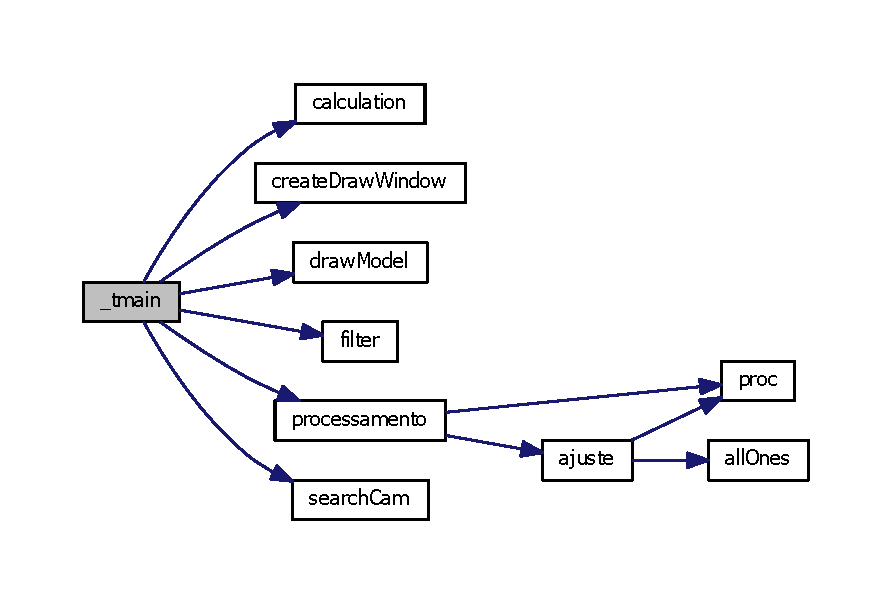
\includegraphics[width=350pt]{main_8cpp_a85563ce6e90d50877f86d857c9f57eb9_cgraph}
\end{center}
\end{figure}


\hypertarget{main_8cpp_adec1dced023c091070e2ea77058e824d}{\index{main.\-cpp@{main.\-cpp}!ajuste@{ajuste}}
\index{ajuste@{ajuste}!main.cpp@{main.\-cpp}}
\subsubsection[{ajuste}]{\setlength{\rightskip}{0pt plus 5cm}void ajuste (
\begin{DoxyParamCaption}
\item[{int}]{Vc\-Size, }
\item[{Range}]{Mat\-Row\mbox{[}$\,$\mbox{]}, }
\item[{Range}]{Mat\-Col\mbox{[}$\,$\mbox{]}, }
\item[{int $\ast$}]{properties\mbox{[}$\,$\mbox{]}, }
\item[{Mat \&}]{src, }
\item[{Mat \&}]{dst}
\end{DoxyParamCaption}
)}}\label{main_8cpp_adec1dced023c091070e2ea77058e824d}


Definition at line 462 of file main.\-cpp.



References all\-Ones(), max\-Points, P\-R\-E\-C\-I\-S\-A\-O\-\_\-\-B\-U\-S\-C\-A, and proc().



Referenced by processamento().


\begin{DoxyCode}
462                                                                                                \{
463     Mat VcMat[\hyperlink{main_8cpp_a7f59d98329dcda0cc22da8a60dda7d2a}{maxPoints}];
464 
465     \textcolor{keywordflow}{if} (VcSize == 0) \{
466         cout << \textcolor{stringliteral}{"VcSize = 0\(\backslash\)n"};
467         \textcolor{keywordflow}{return};
468     \}
469     
470     \textcolor{keywordtype}{int} u = 0;
471     \textcolor{comment}{//Os minimos primeiro}
472     \textcolor{keywordflow}{while}(u < 3) \{
473         \textcolor{comment}{//Incrementa a primeira propriedade}
474         *properties[u] += 1;
475         \hyperlink{main_8cpp_a3cacad06336486e3053a3cd8bdebe09e}{proc}(src,dst);
476 
477         \textcolor{comment}{//Seleciona todas as imagens}
478         \textcolor{keywordflow}{for} (\textcolor{keywordtype}{int} y = 0; y < VcSize; y++) \{
479             VcMat[y] = dst(MatRow[y],MatCol[y]);
480         \}
481 
482         \textcolor{comment}{//Verifica se as imagens estao de acordo}
483         \textcolor{keywordflow}{if}(!\hyperlink{main_8cpp_a485725f864aa7ae9633b72eb64bcd35d}{allOnes}(VcMat,VcSize,\hyperlink{main_8cpp_a2229eef9ff33e056dadf45c70f222814}{PRECISAO\_BUSCA})) \{
484             *properties[u] -= 1;
485             \hyperlink{main_8cpp_a3cacad06336486e3053a3cd8bdebe09e}{proc}(src,dst);
486             \textcolor{keywordflow}{for} (\textcolor{keywordtype}{int} y = 0; y < VcSize; y++) \{
487                 VcMat[y] = dst(MatRow[y],MatCol[y]);
488             \}
489             u += 1;
490         \}
491     \}
492     \textcolor{comment}{//mesmos passos da anterior, mas para os valores maximos}
493     \textcolor{keywordflow}{while} (u < 6) \{
494         *properties[u] -= 1;
495         \hyperlink{main_8cpp_a3cacad06336486e3053a3cd8bdebe09e}{proc}(src,dst);
496         \textcolor{keywordflow}{for} (\textcolor{keywordtype}{int} y = 0; y < VcSize; y++) \{
497             VcMat[y] = dst(MatRow[y],MatCol[y]);
498         \}
499         \textcolor{keywordflow}{if}(!\hyperlink{main_8cpp_a485725f864aa7ae9633b72eb64bcd35d}{allOnes}(VcMat,VcSize,\hyperlink{main_8cpp_a2229eef9ff33e056dadf45c70f222814}{PRECISAO\_BUSCA})) \{
500             *properties[u] += 1;
501             \hyperlink{main_8cpp_a3cacad06336486e3053a3cd8bdebe09e}{proc}(src,dst);
502             \textcolor{keywordflow}{for} (\textcolor{keywordtype}{int} y = 0; y < VcSize; y++) \{
503                 VcMat[y] = dst(MatRow[y],MatCol[y]);
504             \}
505             u += 1;
506         \}
507     \}
508 \}
\end{DoxyCode}


Here is the call graph for this function\-:
\nopagebreak
\begin{figure}[H]
\begin{center}
\leavevmode
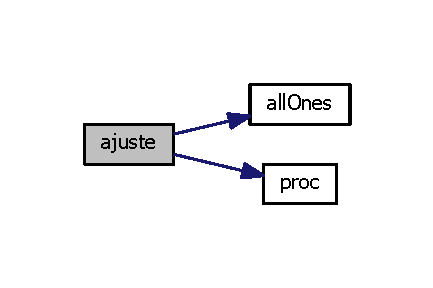
\includegraphics[width=208pt]{main_8cpp_adec1dced023c091070e2ea77058e824d_cgraph}
\end{center}
\end{figure}




Here is the caller graph for this function\-:
\nopagebreak
\begin{figure}[H]
\begin{center}
\leavevmode
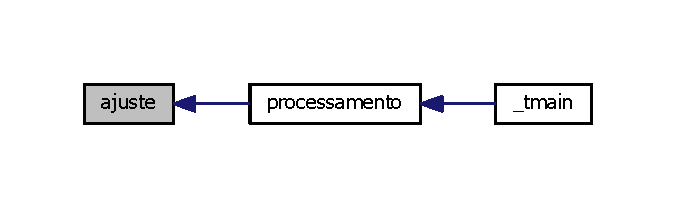
\includegraphics[width=324pt]{main_8cpp_adec1dced023c091070e2ea77058e824d_icgraph}
\end{center}
\end{figure}


\hypertarget{main_8cpp_a485725f864aa7ae9633b72eb64bcd35d}{\index{main.\-cpp@{main.\-cpp}!all\-Ones@{all\-Ones}}
\index{all\-Ones@{all\-Ones}!main.cpp@{main.\-cpp}}
\subsubsection[{all\-Ones}]{\setlength{\rightskip}{0pt plus 5cm}bool all\-Ones (
\begin{DoxyParamCaption}
\item[{Mat}]{Vc\-Mat\mbox{[}$\,$\mbox{]}, }
\item[{int}]{Vc\-Size, }
\item[{int}]{num\-Elements}
\end{DoxyParamCaption}
)}}\label{main_8cpp_a485725f864aa7ae9633b72eb64bcd35d}


Definition at line 443 of file main.\-cpp.



Referenced by ajuste().


\begin{DoxyCode}
443                                                        \{
444     \textcolor{keywordtype}{bool} res = \textcolor{keyword}{true};
445     \textcolor{keywordflow}{for}(\textcolor{keywordtype}{int} z = 0; z < VcSize; z++) \{
446         \textcolor{keywordflow}{if}(countNonZero(VcMat[z]) < numElements) \{
447             res = \textcolor{keyword}{false};
448             \textcolor{keywordflow}{break};
449         \}
450     \}
451     \textcolor{keywordflow}{return} res;
452 \}
\end{DoxyCode}


Here is the caller graph for this function\-:
\nopagebreak
\begin{figure}[H]
\begin{center}
\leavevmode
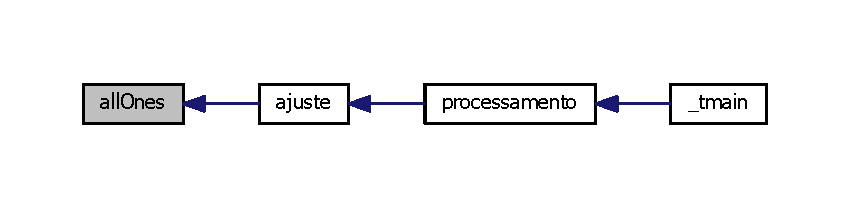
\includegraphics[width=350pt]{main_8cpp_a485725f864aa7ae9633b72eb64bcd35d_icgraph}
\end{center}
\end{figure}


\hypertarget{main_8cpp_a2eda67e2586d9cd56c494f02239c73e9}{\index{main.\-cpp@{main.\-cpp}!calculation@{calculation}}
\index{calculation@{calculation}!main.cpp@{main.\-cpp}}
\subsubsection[{calculation}]{\setlength{\rightskip}{0pt plus 5cm}double calculation (
\begin{DoxyParamCaption}
\item[{vector$<$ vector$<$ Point $>$$>$}]{region, }
\item[{Mat}]{image}
\end{DoxyParamCaption}
)}}\label{main_8cpp_a2eda67e2586d9cd56c494f02239c73e9}


Definition at line 562 of file main.\-cpp.



Referenced by \-\_\-tmain().


\begin{DoxyCode}
562                                                             \{
563     \textcolor{keywordflow}{if}( !region.empty() ) \{
564         Mat bin = Mat::zeros(image.rows,image.cols,CV\_8UC1);
565         drawContours(bin,region,0,Scalar(255),-1);
566         Scalar mean,stdd;
567         meanStdDev(image,mean,stdd,bin);
568         cout << mean << endl << stdd << endl;
569         \textcolor{keywordflow}{return} (mean[1] + 2*stdd[1]);
570     \}
571 
572     \textcolor{keywordflow}{else}
573         \textcolor{keywordflow}{return} 0;
574 \}\end{DoxyCode}


Here is the caller graph for this function\-:
\nopagebreak
\begin{figure}[H]
\begin{center}
\leavevmode
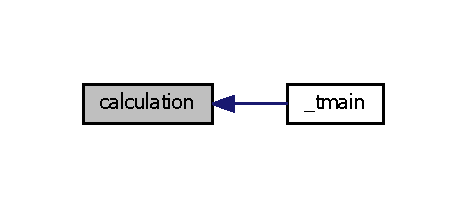
\includegraphics[width=224pt]{main_8cpp_a2eda67e2586d9cd56c494f02239c73e9_icgraph}
\end{center}
\end{figure}


\hypertarget{main_8cpp_a2c80bf65c83f15c94722f105aa99f9ac}{\index{main.\-cpp@{main.\-cpp}!create\-Draw\-Window@{create\-Draw\-Window}}
\index{create\-Draw\-Window@{create\-Draw\-Window}!main.cpp@{main.\-cpp}}
\subsubsection[{create\-Draw\-Window}]{\setlength{\rightskip}{0pt plus 5cm}void create\-Draw\-Window (
\begin{DoxyParamCaption}
\item[{string}]{name, }
\item[{string}]{type}
\end{DoxyParamCaption}
)}}\label{main_8cpp_a2c80bf65c83f15c94722f105aa99f9ac}


Definition at line 347 of file main.\-cpp.



References base, font\-Face, height, left\-\_\-text, M\-A\-X\-\_\-\-D\-R\-A\-W\-I\-N\-G\-\_\-\-C\-I\-R\-C\-L\-E\-\_\-\-R\-A\-D\-I\-U\-S, M\-A\-X\-\_\-\-D\-R\-A\-W\-I\-N\-G\-\_\-\-R\-E\-C\-T\-\_\-\-B\-A\-S\-E, M\-A\-X\-\_\-\-D\-R\-A\-W\-I\-N\-G\-\_\-\-R\-E\-C\-T\-\_\-\-H\-E\-I\-G\-H\-T, M\-A\-X\-\_\-\-F\-O\-N\-T\-\_\-\-S\-C\-A\-L\-E, M\-A\-X\-\_\-\-F\-O\-N\-T\-\_\-\-T\-Y\-P\-E, M\-A\-X\-\_\-\-T\-E\-X\-T\-\_\-\-O\-F\-F\-S\-E\-T, offset\-X, offset\-Y, radius, scale, size\-Cols, size\-Rows, text\-\_\-offset\-X, text\-\_\-offset\-Y, T\-Y\-P\-E\-\_\-\-C\-I\-R\-C\-L\-E, and T\-Y\-P\-E\-\_\-\-R\-E\-C\-T.



Referenced by \-\_\-tmain().


\begin{DoxyCode}
347                                                   \{
348     \textcolor{comment}{//Janela para as configuracoes do modelo com barras para altera-las}
349     namedWindow(name,CV\_WINDOW\_FREERATIO);
350     
351     \textcolor{comment}{//Se o modelo e um retangulo}
352     \textcolor{keywordflow}{if} (\hyperlink{main_8cpp_acce15679d830831b0bbe8ebc2a60b2ca}{type} == \hyperlink{main_8cpp_a8f71c795785904163fae8bf2510fa686}{TYPE\_RECT}) \{
353         createTrackbar(\textcolor{stringliteral}{"Base"},name,&\hyperlink{main_8cpp_a19437a5875428e719515fb20de8a6927}{base},\hyperlink{main_8cpp_a0d5912f74422df9b327467244e45f38b}{MAX\_DRAWING\_RECT\_BASE});       \textcolor{comment}{//Base do
       retangulo}
354         createTrackbar(\textcolor{stringliteral}{"Height"},name,&\hyperlink{main_8cpp_ad12fc34ce789bce6c8a05d8a17138534}{height},\hyperlink{main_8cpp_a6d1f72c1dc90c48752f43f4a90fc5902}{MAX\_DRAWING\_RECT\_HEIGHT}); \textcolor{comment}{//
      Altura do retangulo}
355     \}
356     \textcolor{comment}{//Se o modelo e um circulo}
357     \textcolor{keywordflow}{else} \textcolor{keywordflow}{if} (\hyperlink{main_8cpp_acce15679d830831b0bbe8ebc2a60b2ca}{type} == \hyperlink{main_8cpp_a2234930167879eb15de58567a2615fa4}{TYPE\_CIRCLE}) \{
358         createTrackbar(\textcolor{stringliteral}{"Radius"},name,&\hyperlink{main_8cpp_a395279899207ce7f17adf9fdb8ee97ee}{radius},\hyperlink{main_8cpp_ad9b4a183f843f4b4c60de13e04624fe9}{MAX\_DRAWING\_CIRCLE\_RADIUS});\textcolor{comment}{//
      Raio do ciruclo}
359     \}
360 
361     createTrackbar(\textcolor{stringliteral}{"offsetX"},name,&\hyperlink{main_8cpp_a57abafae3e09830d3569389b2cfcd6d5}{offsetX},\hyperlink{main_8cpp_a931521bf226b983dbf1b2c40ee56eec7}{sizeCols});                    \textcolor{comment}{//Offset X do
       centro}
362     createTrackbar(\textcolor{stringliteral}{"offsety"},name,&\hyperlink{main_8cpp_ad187214e7b10f8e8d3d271c33dbdb91f}{offsetY},\hyperlink{main_8cpp_a17cd3d9778d66fe6033661fcdd2d2b63}{sizeRows});                    \textcolor{comment}{//Offset Y do
       centro}
363     createTrackbar(\textcolor{stringliteral}{"Text X"},name,&\hyperlink{main_8cpp_a76c9a710cb974965ba690749726bdc1d}{text\_offsetX},\hyperlink{main_8cpp_a82ffc259b8582be3bd639da25ce880ab}{MAX\_TEXT\_OFFSET});     \textcolor{comment}{//Offset X
       do texto}
364     createTrackbar(\textcolor{stringliteral}{"Text Y"},name,&\hyperlink{main_8cpp_ac6035bf74a571f9ad49eefc8823d9537}{text\_offsetY},\hyperlink{main_8cpp_a82ffc259b8582be3bd639da25ce880ab}{MAX\_TEXT\_OFFSET});     \textcolor{comment}{//Offset Y
       do texto}
365     createTrackbar(\textcolor{stringliteral}{"left\_text"},name,&\hyperlink{main_8cpp_a86a8ba108d7d4273bf15c0f97f67b7cb}{left\_text},\hyperlink{main_8cpp_a82ffc259b8582be3bd639da25ce880ab}{MAX\_TEXT\_OFFSET});        \textcolor{comment}{//Offset X
       adicional do texto esquerdo}
366     createTrackbar(\textcolor{stringliteral}{"fontFace"},name,&\hyperlink{main_8cpp_a63d30e1b4d55827d6df4f95076af5d43}{fontFace},\hyperlink{main_8cpp_ac2ac25a24068091b377a725810e748ec}{MAX\_FONT\_TYPE});           \textcolor{comment}{//Fonte do
       texto}
367     createTrackbar(\textcolor{stringliteral}{"scale"},name,&\hyperlink{main_8cpp_a418e7934b5363ecde8269070181b3cef}{scale},\hyperlink{main_8cpp_a24ddddae4a965d15b721a59f224cddbb}{MAX\_FONT\_SCALE});                  \textcolor{comment}{//Tamanho do
       texto}
368 
369     \textcolor{keywordflow}{return};
370 \}
\end{DoxyCode}


Here is the caller graph for this function\-:
\nopagebreak
\begin{figure}[H]
\begin{center}
\leavevmode
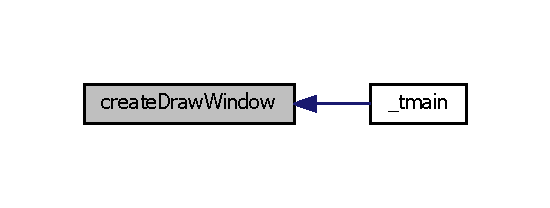
\includegraphics[width=264pt]{main_8cpp_a2c80bf65c83f15c94722f105aa99f9ac_icgraph}
\end{center}
\end{figure}


\hypertarget{main_8cpp_aff29bef05524fd9d6b93d005a927e128}{\index{main.\-cpp@{main.\-cpp}!draw\-Model@{draw\-Model}}
\index{draw\-Model@{draw\-Model}!main.cpp@{main.\-cpp}}
\subsubsection[{draw\-Model}]{\setlength{\rightskip}{0pt plus 5cm}Mat draw\-Model (
\begin{DoxyParamCaption}
\item[{string}]{type, }
\item[{Mat}]{image}
\end{DoxyParamCaption}
)}}\label{main_8cpp_aff29bef05524fd9d6b93d005a927e128}


Definition at line 372 of file main.\-cpp.



References base, font\-Face, F\-U\-L\-L\-\_\-\-W\-H\-E\-I\-G\-H\-T, height, left\-\_\-text, N\-O\-\_\-\-W\-H\-E\-I\-G\-H\-T, offset\-X, offset\-Y, O\-F\-F\-S\-E\-T\-Y\-\_\-2\-R\-E\-C\-T, O\-U\-T\-L\-I\-N\-E\-\_\-\-C\-O\-L\-O\-R, O\-U\-T\-L\-I\-N\-E\-\_\-\-T\-H\-I\-C\-K\-N\-E\-S\-S, radius, scale, text\-\_\-offset\-X, text\-\_\-offset\-Y, T\-E\-X\-T\-\_\-\-T\-H\-I\-C\-K\-N\-E\-S\-S, T\-H\-R\-E\-E\-\_\-\-F\-O\-U\-R\-T\-H\-S\-\_\-\-W\-H\-E\-I\-G\-H\-T, T\-Y\-P\-E\-\_\-\-C\-I\-R\-C\-L\-E, T\-Y\-P\-E\-\_\-\-R\-E\-C\-T, and T\-Y\-P\-E\-\_\-\-R\-E\-C\-T2.



Referenced by \-\_\-tmain().


\begin{DoxyCode}
372                                       \{
373     \textcolor{comment}{//Initialize drawing to all black.}
374     Mat drawing = Mat::zeros(image.rows,image.cols,CV\_8UC3);
375     
376     
377     \textcolor{keywordflow}{if} (\hyperlink{main_8cpp_acce15679d830831b0bbe8ebc2a60b2ca}{type} == \hyperlink{main_8cpp_a2234930167879eb15de58567a2615fa4}{TYPE\_CIRCLE}) \{
378         \textcolor{comment}{//Draws a circle in drawing.}
379         circle(drawing,Point(\hyperlink{main_8cpp_a57abafae3e09830d3569389b2cfcd6d5}{offsetX},\hyperlink{main_8cpp_ad187214e7b10f8e8d3d271c33dbdb91f}{offsetY}),\hyperlink{main_8cpp_a395279899207ce7f17adf9fdb8ee97ee}{radius},
      \hyperlink{main_8cpp_ac67bb96add6ae84d267d9a8f270a6142}{OUTLINE\_COLOR},\hyperlink{main_8cpp_adde6da43045ef2137942ae981e4f13ca}{OUTLINE\_THICKNESS});
380 
381         \textcolor{comment}{//Draws the vertical middle line of the circle.}
382         line(drawing,Point(\hyperlink{main_8cpp_a57abafae3e09830d3569389b2cfcd6d5}{offsetX},(\hyperlink{main_8cpp_ad187214e7b10f8e8d3d271c33dbdb91f}{offsetY}-\hyperlink{main_8cpp_a395279899207ce7f17adf9fdb8ee97ee}{radius})),Point(
      \hyperlink{main_8cpp_a57abafae3e09830d3569389b2cfcd6d5}{offsetX},(\hyperlink{main_8cpp_ad187214e7b10f8e8d3d271c33dbdb91f}{offsetY}+\hyperlink{main_8cpp_a395279899207ce7f17adf9fdb8ee97ee}{radius})),\hyperlink{main_8cpp_ac67bb96add6ae84d267d9a8f270a6142}{OUTLINE\_COLOR},
      \hyperlink{main_8cpp_adde6da43045ef2137942ae981e4f13ca}{OUTLINE\_THICKNESS});
383 
384         \textcolor{comment}{//Write text.}
385         putText(drawing,\textcolor{stringliteral}{"C"},Point((\hyperlink{main_8cpp_a57abafae3e09830d3569389b2cfcd6d5}{offsetX}-\hyperlink{main_8cpp_a395279899207ce7f17adf9fdb8ee97ee}{radius}-\hyperlink{main_8cpp_a76c9a710cb974965ba690749726bdc1d}{text\_offsetX}-
      \hyperlink{main_8cpp_a86a8ba108d7d4273bf15c0f97f67b7cb}{left\_text}),(\hyperlink{main_8cpp_ad187214e7b10f8e8d3d271c33dbdb91f}{offsetY}+\hyperlink{main_8cpp_ac6035bf74a571f9ad49eefc8823d9537}{text\_offsetY})),\hyperlink{main_8cpp_a63d30e1b4d55827d6df4f95076af5d43}{fontFace},
      \hyperlink{main_8cpp_a418e7934b5363ecde8269070181b3cef}{scale}/10.0,\hyperlink{main_8cpp_ac67bb96add6ae84d267d9a8f270a6142}{OUTLINE\_COLOR},\hyperlink{main_8cpp_ab68e4b3d804fc8781d01aca817a71c1e}{TEXT\_THICKNESS});
386         putText(drawing,\textcolor{stringliteral}{"T"},Point((\hyperlink{main_8cpp_a57abafae3e09830d3569389b2cfcd6d5}{offsetX}+\hyperlink{main_8cpp_a395279899207ce7f17adf9fdb8ee97ee}{radius}+\hyperlink{main_8cpp_a76c9a710cb974965ba690749726bdc1d}{text\_offsetX}),(
      \hyperlink{main_8cpp_ad187214e7b10f8e8d3d271c33dbdb91f}{offsetY}+\hyperlink{main_8cpp_ac6035bf74a571f9ad49eefc8823d9537}{text\_offsetY})),\hyperlink{main_8cpp_a63d30e1b4d55827d6df4f95076af5d43}{fontFace},\hyperlink{main_8cpp_a418e7934b5363ecde8269070181b3cef}{scale}/10.0,
      \hyperlink{main_8cpp_ac67bb96add6ae84d267d9a8f270a6142}{OUTLINE\_COLOR},\hyperlink{main_8cpp_ab68e4b3d804fc8781d01aca817a71c1e}{TEXT\_THICKNESS});
387     \}
388     
389     \textcolor{keywordflow}{else} \textcolor{keywordflow}{if} (\hyperlink{main_8cpp_acce15679d830831b0bbe8ebc2a60b2ca}{type} == \hyperlink{main_8cpp_a8f71c795785904163fae8bf2510fa686}{TYPE\_RECT}) \{
390         \textcolor{comment}{//Draws a rectangle in drawing.}
391         rectangle(drawing,Point(\hyperlink{main_8cpp_a57abafae3e09830d3569389b2cfcd6d5}{offsetX}-\hyperlink{main_8cpp_a19437a5875428e719515fb20de8a6927}{base}/2,\hyperlink{main_8cpp_ad187214e7b10f8e8d3d271c33dbdb91f}{offsetY}-\hyperlink{main_8cpp_ad12fc34ce789bce6c8a05d8a17138534}{height}/2),Point(
      \hyperlink{main_8cpp_a57abafae3e09830d3569389b2cfcd6d5}{offsetX}+\hyperlink{main_8cpp_a19437a5875428e719515fb20de8a6927}{base}/2,\hyperlink{main_8cpp_ad187214e7b10f8e8d3d271c33dbdb91f}{offsetY}+\hyperlink{main_8cpp_ad12fc34ce789bce6c8a05d8a17138534}{height}/2),Scalar(0,255,0),
      \hyperlink{main_8cpp_adde6da43045ef2137942ae981e4f13ca}{OUTLINE\_THICKNESS});
392         
393         \textcolor{comment}{//Draws the vertical middle line of the rectangle.}
394         line(drawing,Point(\hyperlink{main_8cpp_a57abafae3e09830d3569389b2cfcd6d5}{offsetX},(\hyperlink{main_8cpp_ad187214e7b10f8e8d3d271c33dbdb91f}{offsetY}-\hyperlink{main_8cpp_ad12fc34ce789bce6c8a05d8a17138534}{height}/2)),Point(
      \hyperlink{main_8cpp_a57abafae3e09830d3569389b2cfcd6d5}{offsetX},(\hyperlink{main_8cpp_ad187214e7b10f8e8d3d271c33dbdb91f}{offsetY}+\hyperlink{main_8cpp_ad12fc34ce789bce6c8a05d8a17138534}{height}/2)),\hyperlink{main_8cpp_ac67bb96add6ae84d267d9a8f270a6142}{OUTLINE\_COLOR},
      \hyperlink{main_8cpp_adde6da43045ef2137942ae981e4f13ca}{OUTLINE\_THICKNESS});
395         
396         \textcolor{comment}{//Write text.}
397         putText(drawing,\textcolor{stringliteral}{"C"},Point((\hyperlink{main_8cpp_a57abafae3e09830d3569389b2cfcd6d5}{offsetX}-\hyperlink{main_8cpp_a19437a5875428e719515fb20de8a6927}{base}/2-\hyperlink{main_8cpp_a76c9a710cb974965ba690749726bdc1d}{text\_offsetX}-
      \hyperlink{main_8cpp_a86a8ba108d7d4273bf15c0f97f67b7cb}{left\_text}),(\hyperlink{main_8cpp_ad187214e7b10f8e8d3d271c33dbdb91f}{offsetY}+\hyperlink{main_8cpp_ac6035bf74a571f9ad49eefc8823d9537}{text\_offsetY})),\hyperlink{main_8cpp_a63d30e1b4d55827d6df4f95076af5d43}{fontFace},
      \hyperlink{main_8cpp_a418e7934b5363ecde8269070181b3cef}{scale}/10.0,\hyperlink{main_8cpp_ac67bb96add6ae84d267d9a8f270a6142}{OUTLINE\_COLOR},\hyperlink{main_8cpp_ab68e4b3d804fc8781d01aca817a71c1e}{TEXT\_THICKNESS});
398         putText(drawing,\textcolor{stringliteral}{"T"},Point((\hyperlink{main_8cpp_a57abafae3e09830d3569389b2cfcd6d5}{offsetX}+\hyperlink{main_8cpp_a19437a5875428e719515fb20de8a6927}{base}/2+\hyperlink{main_8cpp_a76c9a710cb974965ba690749726bdc1d}{text\_offsetX}),(
      \hyperlink{main_8cpp_ad187214e7b10f8e8d3d271c33dbdb91f}{offsetY}+\hyperlink{main_8cpp_ac6035bf74a571f9ad49eefc8823d9537}{text\_offsetY})),\hyperlink{main_8cpp_a63d30e1b4d55827d6df4f95076af5d43}{fontFace},\hyperlink{main_8cpp_a418e7934b5363ecde8269070181b3cef}{scale}/10.0,
      \hyperlink{main_8cpp_ac67bb96add6ae84d267d9a8f270a6142}{OUTLINE\_COLOR},\hyperlink{main_8cpp_ab68e4b3d804fc8781d01aca817a71c1e}{TEXT\_THICKNESS});
399 
400     \}
401 
402     \textcolor{keywordflow}{else} \textcolor{keywordflow}{if} (\hyperlink{main_8cpp_acce15679d830831b0bbe8ebc2a60b2ca}{type} == \hyperlink{main_8cpp_ae6102eb5288b8f5e0d6ef03190842b1b}{TYPE\_RECT2}) \{
403         \textcolor{comment}{//Draws a rectangle in drawing.}
404         rectangle(drawing,Point(\hyperlink{main_8cpp_a57abafae3e09830d3569389b2cfcd6d5}{offsetX}-\hyperlink{main_8cpp_a19437a5875428e719515fb20de8a6927}{base}/2,\hyperlink{main_8cpp_ad187214e7b10f8e8d3d271c33dbdb91f}{offsetY}-\hyperlink{main_8cpp_ad12fc34ce789bce6c8a05d8a17138534}{height}/2 - 
      \hyperlink{main_8cpp_a105decd3af846926e9dd6edb4fb327b8}{OFFSETY\_2RECT}),Point(\hyperlink{main_8cpp_a57abafae3e09830d3569389b2cfcd6d5}{offsetX}+\hyperlink{main_8cpp_a19437a5875428e719515fb20de8a6927}{base}/2,\hyperlink{main_8cpp_ad187214e7b10f8e8d3d271c33dbdb91f}{offsetY}+
      \hyperlink{main_8cpp_ad12fc34ce789bce6c8a05d8a17138534}{height}/2 - \hyperlink{main_8cpp_a105decd3af846926e9dd6edb4fb327b8}{OFFSETY\_2RECT}),Scalar(0,255,0),\hyperlink{main_8cpp_adde6da43045ef2137942ae981e4f13ca}{OUTLINE\_THICKNESS});
405         
406         \textcolor{comment}{//Draws the vertical middle line of the rectangle.}
407         line(drawing,Point(\hyperlink{main_8cpp_a57abafae3e09830d3569389b2cfcd6d5}{offsetX},(\hyperlink{main_8cpp_ad187214e7b10f8e8d3d271c33dbdb91f}{offsetY}-\hyperlink{main_8cpp_ad12fc34ce789bce6c8a05d8a17138534}{height}/2 - 
      \hyperlink{main_8cpp_a105decd3af846926e9dd6edb4fb327b8}{OFFSETY\_2RECT})),Point(\hyperlink{main_8cpp_a57abafae3e09830d3569389b2cfcd6d5}{offsetX},(\hyperlink{main_8cpp_ad187214e7b10f8e8d3d271c33dbdb91f}{offsetY}+\hyperlink{main_8cpp_ad12fc34ce789bce6c8a05d8a17138534}{height}/2-
      \hyperlink{main_8cpp_a105decd3af846926e9dd6edb4fb327b8}{OFFSETY\_2RECT})),\hyperlink{main_8cpp_ac67bb96add6ae84d267d9a8f270a6142}{OUTLINE\_COLOR},\hyperlink{main_8cpp_adde6da43045ef2137942ae981e4f13ca}{OUTLINE\_THICKNESS});
408         
409         \textcolor{comment}{//Write text.}
410         putText(drawing,\textcolor{stringliteral}{"C"},Point((\hyperlink{main_8cpp_a57abafae3e09830d3569389b2cfcd6d5}{offsetX}-\hyperlink{main_8cpp_a19437a5875428e719515fb20de8a6927}{base}/2-\hyperlink{main_8cpp_a76c9a710cb974965ba690749726bdc1d}{text\_offsetX}-
      \hyperlink{main_8cpp_a86a8ba108d7d4273bf15c0f97f67b7cb}{left\_text}),(\hyperlink{main_8cpp_ad187214e7b10f8e8d3d271c33dbdb91f}{offsetY}+\hyperlink{main_8cpp_ac6035bf74a571f9ad49eefc8823d9537}{text\_offsetY}-\hyperlink{main_8cpp_a105decd3af846926e9dd6edb4fb327b8}{OFFSETY\_2RECT})),
      \hyperlink{main_8cpp_a63d30e1b4d55827d6df4f95076af5d43}{fontFace},\hyperlink{main_8cpp_a418e7934b5363ecde8269070181b3cef}{scale}/10.0,\hyperlink{main_8cpp_ac67bb96add6ae84d267d9a8f270a6142}{OUTLINE\_COLOR},\hyperlink{main_8cpp_ab68e4b3d804fc8781d01aca817a71c1e}{TEXT\_THICKNESS});
411         putText(drawing,\textcolor{stringliteral}{"T"},Point((\hyperlink{main_8cpp_a57abafae3e09830d3569389b2cfcd6d5}{offsetX}+\hyperlink{main_8cpp_a19437a5875428e719515fb20de8a6927}{base}/2+\hyperlink{main_8cpp_a76c9a710cb974965ba690749726bdc1d}{text\_offsetX}),(
      \hyperlink{main_8cpp_ad187214e7b10f8e8d3d271c33dbdb91f}{offsetY}+\hyperlink{main_8cpp_ac6035bf74a571f9ad49eefc8823d9537}{text\_offsetY}-\hyperlink{main_8cpp_a105decd3af846926e9dd6edb4fb327b8}{OFFSETY\_2RECT})),\hyperlink{main_8cpp_a63d30e1b4d55827d6df4f95076af5d43}{fontFace},
      \hyperlink{main_8cpp_a418e7934b5363ecde8269070181b3cef}{scale}/10.0,\hyperlink{main_8cpp_ac67bb96add6ae84d267d9a8f270a6142}{OUTLINE\_COLOR},\hyperlink{main_8cpp_ab68e4b3d804fc8781d01aca817a71c1e}{TEXT\_THICKNESS});
412 
413     \}
414     
415     \textcolor{comment}{//Add the actual frame with the drawing, forming a new image.}
416     addWeighted(image,\hyperlink{main_8cpp_a9a9b6184443622ad50fd17dbc3d006a6}{FULL\_WHEIGHT},drawing,\hyperlink{main_8cpp_a0feaa74b2b5e463d13bd697f8bbd6b24}{THREE\_FOURTHS\_WHEIGHT},
      \hyperlink{main_8cpp_a7c5c9e6093f80f0676571c239290dda1}{NO\_WHEIGHT},image);
417 
418 
419     \textcolor{keywordflow}{return} image;
420 \}
\end{DoxyCode}


Here is the caller graph for this function\-:
\nopagebreak
\begin{figure}[H]
\begin{center}
\leavevmode
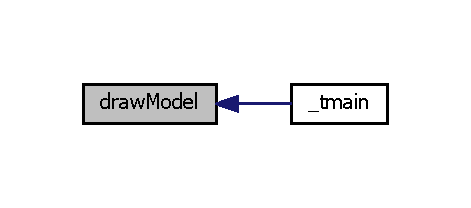
\includegraphics[width=226pt]{main_8cpp_aff29bef05524fd9d6b93d005a927e128_icgraph}
\end{center}
\end{figure}


\hypertarget{main_8cpp_a34ccd5a5f5e6c89511ed19c070eb3206}{\index{main.\-cpp@{main.\-cpp}!filter@{filter}}
\index{filter@{filter}!main.cpp@{main.\-cpp}}
\subsubsection[{filter}]{\setlength{\rightskip}{0pt plus 5cm}void filter (
\begin{DoxyParamCaption}
\item[{Mat \&}]{src, }
\item[{Mat \&}]{dst}
\end{DoxyParamCaption}
)}}\label{main_8cpp_a34ccd5a5f5e6c89511ed19c070eb3206}


Definition at line 422 of file main.\-cpp.



References \-\_\-sz\-Height, \-\_\-sz\-Width, and delta.



Referenced by \-\_\-tmain().


\begin{DoxyCode}
422                                 \{
423     Size siz(\hyperlink{main_8cpp_a45ad72b14f4530cc2c56e634d1b173d7}{\_szWidth},\hyperlink{main_8cpp_a1cc0e1fd2d4da3a678657cd5be953816}{\_szHeight});
424     GaussianBlur(src,dst,siz,\hyperlink{main_8cpp_a1dfcb70b9229f2da17dd5922b87ecf2c}{delta}/100.0);
425     \textcolor{keywordflow}{return};
426 \}
\end{DoxyCode}


Here is the caller graph for this function\-:
\nopagebreak
\begin{figure}[H]
\begin{center}
\leavevmode
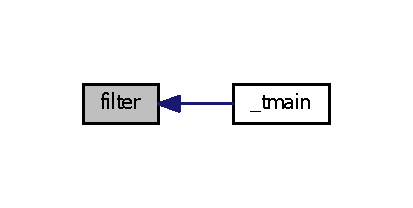
\includegraphics[width=198pt]{main_8cpp_a34ccd5a5f5e6c89511ed19c070eb3206_icgraph}
\end{center}
\end{figure}


\hypertarget{main_8cpp_a3cacad06336486e3053a3cd8bdebe09e}{\index{main.\-cpp@{main.\-cpp}!proc@{proc}}
\index{proc@{proc}!main.cpp@{main.\-cpp}}
\subsubsection[{proc}]{\setlength{\rightskip}{0pt plus 5cm}void proc (
\begin{DoxyParamCaption}
\item[{Mat \&}]{src, }
\item[{Mat \&}]{dst}
\end{DoxyParamCaption}
)}}\label{main_8cpp_a3cacad06336486e3053a3cd8bdebe09e}


Definition at line 428 of file main.\-cpp.



References \-\_\-max\-Hue, \-\_\-max\-Sat, \-\_\-max\-Val, \-\_\-min\-Hue, \-\_\-min\-Sat, and \-\_\-min\-Val.



Referenced by ajuste(), and processamento().


\begin{DoxyCode}
428                               \{
429     inRange(src,Scalar(\hyperlink{main_8cpp_a6c156a8f03f7d70255416c642bee7713}{\_minHue},\hyperlink{main_8cpp_a963e41924775b4d345671ae91326338d}{\_minSat},\hyperlink{main_8cpp_ae8a1bd1a611103f5cda9e05c9996e0e7}{\_minVal}),Scalar(
      \hyperlink{main_8cpp_a7f2d59160b6ec5f28816a5c84c2f0387}{\_maxHue},\hyperlink{main_8cpp_a96d19bd8c6abd3ef02e707bad400c96c}{\_maxSat},\hyperlink{main_8cpp_aaa63c2fcee418d0498758ee5f9b28337}{\_maxVal}),dst);
430     \textcolor{keywordflow}{return};
431 \}
\end{DoxyCode}


Here is the caller graph for this function\-:
\nopagebreak
\begin{figure}[H]
\begin{center}
\leavevmode
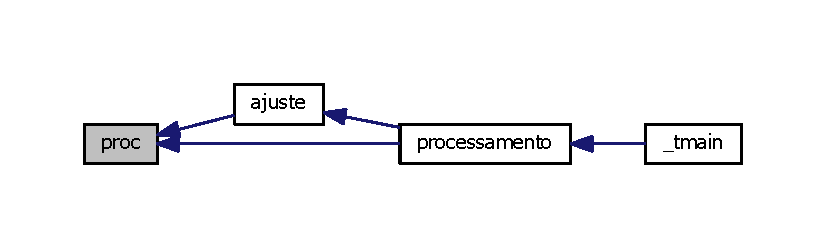
\includegraphics[width=350pt]{main_8cpp_a3cacad06336486e3053a3cd8bdebe09e_icgraph}
\end{center}
\end{figure}


\hypertarget{main_8cpp_ae06205f6d61db52c006bf605c2b2f6f8}{\index{main.\-cpp@{main.\-cpp}!processamento@{processamento}}
\index{processamento@{processamento}!main.cpp@{main.\-cpp}}
\subsubsection[{processamento}]{\setlength{\rightskip}{0pt plus 5cm}vector$<$ vector$<$ Point $>$ $>$ processamento (
\begin{DoxyParamCaption}
\item[{Mat}]{H\-S\-V, }
\item[{Mat}]{bin}
\end{DoxyParamCaption}
)}}\label{main_8cpp_ae06205f6d61db52c006bf605c2b2f6f8}


Definition at line 510 of file main.\-cpp.



References \-\_\-max\-Hue, \-\_\-max\-Sat, \-\_\-max\-Val, \-\_\-min\-Hue, \-\_\-min\-Sat, \-\_\-min\-Val, ajuste(), A\-P\-P\-R\-O\-X\-I\-M\-A\-T\-I\-O\-N, A\-U\-T\-O\-B\-U\-S\-C\-A\-\_\-\-A\-L\-T\-U\-R\-A, A\-U\-T\-O\-B\-U\-S\-C\-A\-\_\-\-L\-A\-R\-G\-U\-R\-A, A\-U\-T\-O\-B\-U\-S\-C\-A\-\_\-\-P\-U\-L\-O, M\-A\-X\-\_\-\-A\-R\-E\-A, max\-Hue, max\-Points, max\-Sat, max\-Val, M\-I\-N\-\_\-\-A\-R\-E\-A, min\-Hue, M\-I\-N\-I\-M\-A\-L\-\_\-\-M\-A\-T\-C\-H, min\-Sat, min\-Val, and proc().



Referenced by \-\_\-tmain().


\begin{DoxyCode}
510                                                       \{
511     \textcolor{keywordtype}{int} *properties[6];
512     Range MatRow[\hyperlink{main_8cpp_a7f59d98329dcda0cc22da8a60dda7d2a}{maxPoints}];
513     Range MatCol[\hyperlink{main_8cpp_a7f59d98329dcda0cc22da8a60dda7d2a}{maxPoints}];
514     \textcolor{keywordtype}{double} match = \hyperlink{main_8cpp_ab996b79d395aa8366c6fafc793c015c4}{MINIMAL\_MATCH},temp;
515     vector<vector<Point>> best;
516     vector<vector<Point>> contours;
517     vector<Point> rect;
518     rect.push\_back(Point(1,1));
519     rect.push\_back(Point(1+\hyperlink{main_8cpp_a4b664b931e7a93cf91809602933c9313}{AUTOBUSCA\_LARGURA},1));
520     rect.push\_back(Point(1+\hyperlink{main_8cpp_a4b664b931e7a93cf91809602933c9313}{AUTOBUSCA\_LARGURA},1+\hyperlink{main_8cpp_af4d22e3468e0e9ff30ea4cc4708bf310}{AUTOBUSCA\_ALTURA}));
521     rect.push\_back(Point(1,1+\hyperlink{main_8cpp_af4d22e3468e0e9ff30ea4cc4708bf310}{AUTOBUSCA\_ALTURA}));
522     rect.push\_back(Point(1,1));
523     properties[0] = &\hyperlink{main_8cpp_a6c156a8f03f7d70255416c642bee7713}{\_minHue}; properties[1] = &\hyperlink{main_8cpp_a963e41924775b4d345671ae91326338d}{\_minSat}; properties[2] = &
      \hyperlink{main_8cpp_ae8a1bd1a611103f5cda9e05c9996e0e7}{\_minVal}; properties[3] = &\hyperlink{main_8cpp_a7f2d59160b6ec5f28816a5c84c2f0387}{\_maxHue}; properties[4] = &\hyperlink{main_8cpp_a96d19bd8c6abd3ef02e707bad400c96c}{\_maxSat}; properties[5] = &
      \hyperlink{main_8cpp_aaa63c2fcee418d0498758ee5f9b28337}{\_maxVal};
524     
525     \textcolor{keywordflow}{for}( \textcolor{keywordtype}{int} ROWS = 0 ; ROWS < HSV.rows - \hyperlink{main_8cpp_af4d22e3468e0e9ff30ea4cc4708bf310}{AUTOBUSCA\_ALTURA}; ROWS+=
      \hyperlink{main_8cpp_a908b1473f4bb5bd5bccb79e90a86554d}{AUTOBUSCA\_PULO}) \{
526         \textcolor{keywordflow}{for}( \textcolor{keywordtype}{int} COLS = 0 ; COLS < HSV.cols - \hyperlink{main_8cpp_a4b664b931e7a93cf91809602933c9313}{AUTOBUSCA\_LARGURA}; COLS+=
      \hyperlink{main_8cpp_a908b1473f4bb5bd5bccb79e90a86554d}{AUTOBUSCA\_PULO}) \{
527                 \hyperlink{main_8cpp_a6c156a8f03f7d70255416c642bee7713}{\_minHue} = \hyperlink{main_8cpp_a86b6713c598f5468273929392532eade}{minHue}; \hyperlink{main_8cpp_a963e41924775b4d345671ae91326338d}{\_minSat} = \hyperlink{main_8cpp_a47c23367137ef58696a7ff35c14a8839}{minSat}; 
      \hyperlink{main_8cpp_ae8a1bd1a611103f5cda9e05c9996e0e7}{\_minVal} = \hyperlink{main_8cpp_a86d9ab7f374e6ea7d65185b705a96628}{minVal}; \hyperlink{main_8cpp_a7f2d59160b6ec5f28816a5c84c2f0387}{\_maxHue} = \hyperlink{main_8cpp_af1c86696d8a09abc6e6d123ba2ae19a9}{maxHue}; \hyperlink{main_8cpp_a96d19bd8c6abd3ef02e707bad400c96c}{\_maxSat} = 
      \hyperlink{main_8cpp_acaadb191360d1bbd61de56a372435c83}{maxSat}; \hyperlink{main_8cpp_aaa63c2fcee418d0498758ee5f9b28337}{\_maxVal} = \hyperlink{main_8cpp_a80484033ea1bd99c5950295c0631cc5b}{maxVal};
528                 \hyperlink{main_8cpp_a3cacad06336486e3053a3cd8bdebe09e}{proc}(HSV,bin);
529                 MatRow[0] = Range(ROWS,ROWS+\hyperlink{main_8cpp_af4d22e3468e0e9ff30ea4cc4708bf310}{AUTOBUSCA\_ALTURA});
530                 MatCol[0] = Range(COLS,COLS+\hyperlink{main_8cpp_a4b664b931e7a93cf91809602933c9313}{AUTOBUSCA\_LARGURA});
531                 
532                 \hyperlink{main_8cpp_adec1dced023c091070e2ea77058e824d}{ajuste}(1,MatRow,MatCol,properties,HSV,bin);
533                 cout << COLS << \textcolor{stringliteral}{" x "} << ROWS << endl;
534         
535                 findContours(bin, contours, CV\_RETR\_EXTERNAL, CV\_CHAIN\_APPROX\_SIMPLE);
536                 cout << \textcolor{stringliteral}{"Found "} << contours.size() << \textcolor{stringliteral}{" contours."} << endl;
537 
538                 \textcolor{keywordflow}{if}(contours.size() == 1 && pointPolygonTest(contours[0],Point2f(COLS,ROWS),\textcolor{keyword}{false}) >= 0) \{
539                     approxPolyDP(contours[0],contours[0],\hyperlink{main_8cpp_aee8c3c363eab49d6a90d3f74587694d5}{APPROXIMATION},\textcolor{keyword}{true});
540                     \textcolor{keywordtype}{double} area = contourArea(contours[0]);
541                     temp = matchShapes(rect,contours[0],CV\_CONTOURS\_MATCH\_I2,0);
542                     cout << temp << endl;
543                     \textcolor{comment}{/*mt = Mat::zeros(mt.rows,mt.cols,CV\_8UC1);}
544 \textcolor{comment}{                    drawContours(mt,contours,0,Scalar(255),-1);}
545 \textcolor{comment}{                    imshow("Detection",mt);}
546 \textcolor{comment}{                    cvtColor(mt,mtRGB,CV\_GRAY2BGR);}
547 \textcolor{comment}{                    show(Trans);*/}
548                     \textcolor{keywordflow}{if}(match > temp && area > \hyperlink{main_8cpp_aa637ca99e2e8b6a736d0910e0f1713bf}{MIN\_AREA} && temp != 0 && area < 
      \hyperlink{main_8cpp_a3d4a6aad8b48293253d708f605965036}{MAX\_AREA}) \{
549                         match = temp;
550                         best.clear();
551                         best.push\_back(contours[0]);
552                         \textcolor{comment}{//if( !best.empty() ) cout << "printed" << endl;}
553                     \}
554                     \textcolor{comment}{//waitKey();}
555                 \}
556             \}
557         \}
558 
559     \textcolor{keywordflow}{return} best;
560 \}
\end{DoxyCode}


Here is the call graph for this function\-:
\nopagebreak
\begin{figure}[H]
\begin{center}
\leavevmode
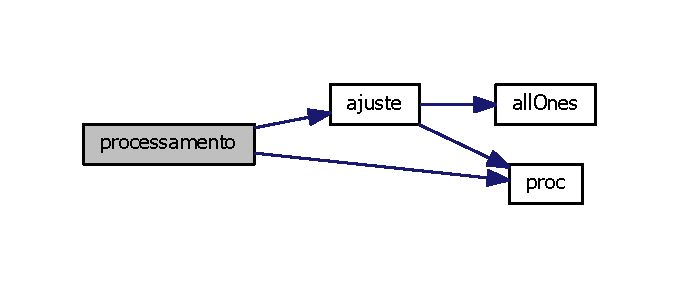
\includegraphics[width=326pt]{main_8cpp_ae06205f6d61db52c006bf605c2b2f6f8_cgraph}
\end{center}
\end{figure}




Here is the caller graph for this function\-:
\nopagebreak
\begin{figure}[H]
\begin{center}
\leavevmode
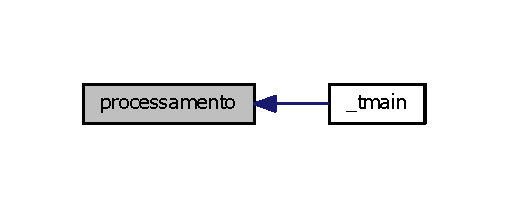
\includegraphics[width=244pt]{main_8cpp_ae06205f6d61db52c006bf605c2b2f6f8_icgraph}
\end{center}
\end{figure}


\hypertarget{main_8cpp_abf53b5314d2e6e573cda0ab847c4f56a}{\index{main.\-cpp@{main.\-cpp}!search\-Cam@{search\-Cam}}
\index{search\-Cam@{search\-Cam}!main.cpp@{main.\-cpp}}
\subsubsection[{search\-Cam}]{\setlength{\rightskip}{0pt plus 5cm}int search\-Cam (
\begin{DoxyParamCaption}
\item[{Video\-Capture $\ast$}]{camera}
\end{DoxyParamCaption}
)}}\label{main_8cpp_abf53b5314d2e6e573cda0ab847c4f56a}


Definition at line 305 of file main.\-cpp.



References E\-R\-R\-\_\-\-N\-O\-\_\-\-C\-A\-M\-E\-R\-A.



Referenced by \-\_\-tmain().


\begin{DoxyCode}
305                                      \{
306     \textcolor{comment}{//Pesquisa todas as cameras possiveis}
307     \textcolor{keywordtype}{int} x,y;
308     \textcolor{keywordflow}{for} (x=0 ; x<10; x++) \{
309         \textcolor{comment}{//Abre a camera.}
310         camera->open(x);
311 
312         \textcolor{comment}{//Se falhar para abrir a camera 'y' sera nosso maximo de cameras.}
313         \textcolor{keywordflow}{if}(!camera->isOpened ()) \{
314             y = x;
315             x += 10;
316         \}
317         \textcolor{comment}{//Se nao falhar continua procurando.}
318         \textcolor{keywordflow}{else} 
319             camera->release();
320     \}
321 
322     \textcolor{comment}{//Caso nao tenha cameras que possam ser usadas ocorre um erro.}
323     \textcolor{keywordflow}{if} (y == 0) \{
324         cout << \textcolor{stringliteral}{"Error "} << \hyperlink{main_8cpp_a6e092cbd5c48e865f9ec561a00cb4475}{ERR\_NO\_CAMERA} << endl;
325         destroyAllWindows();
326         exit (\hyperlink{main_8cpp_a6e092cbd5c48e865f9ec561a00cb4475}{ERR\_NO\_CAMERA});
327     \}
328 
329     \textcolor{comment}{//Mostra as opcoes.}
330     cout << \textcolor{stringliteral}{"Existem "} << y << \textcolor{stringliteral}{" cameras disponiveis.\(\backslash\)n\(\backslash\)nID das cameras:\(\backslash\)n"};
331     \textcolor{keywordflow}{for}(x=0;x<y;x++) cout << x << endl;
332     cout << \textcolor{stringliteral}{"\(\backslash\)nEscolha uma camera para usar.\(\backslash\)n> "};
333 
334     \textcolor{comment}{//Processa a escolha do usuario.}
335     escolha\_camera:
336     cin >> x;
337     \textcolor{keywordflow}{if}(x < 0 || x >= y) \{
338         cout << \textcolor{stringliteral}{"\(\backslash\)nID de camera invalido, tente novamente.\(\backslash\)n> "};
339         \textcolor{keywordflow}{goto} escolha\_camera;
340     \}
341 
342     \textcolor{comment}{//Retorna a camera desejada.}
343     system(\textcolor{stringliteral}{"cls"});
344     \textcolor{keywordflow}{return} x;
345 \}
\end{DoxyCode}


Here is the caller graph for this function\-:
\nopagebreak
\begin{figure}[H]
\begin{center}
\leavevmode
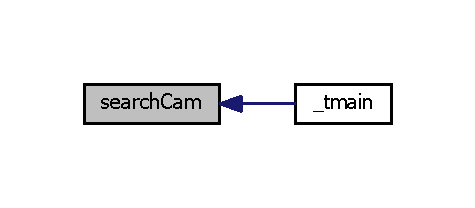
\includegraphics[width=228pt]{main_8cpp_abf53b5314d2e6e573cda0ab847c4f56a_icgraph}
\end{center}
\end{figure}


\hypertarget{main_8cpp_a522a59e6315224b9a413b3e06d5bd6ae}{\index{main.\-cpp@{main.\-cpp}!show@{show}}
\index{show@{show}!main.cpp@{main.\-cpp}}
\subsubsection[{show}]{\setlength{\rightskip}{0pt plus 5cm}Mat show (
\begin{DoxyParamCaption}
\item[{Mat}]{src1, }
\item[{Mat}]{src2, }
\item[{int}]{percentage}
\end{DoxyParamCaption}
)}}\label{main_8cpp_a522a59e6315224b9a413b3e06d5bd6ae}


Definition at line 434 of file main.\-cpp.


\begin{DoxyCode}
434                                              \{
435     Mat result;
436     addWeighted(src1,percentage/100.0,src2,(100-percentage)/100.0,0.0,result);
437     \textcolor{keywordflow}{return} result;
438 \}
\end{DoxyCode}


\subsection{Variable Documentation}
\hypertarget{main_8cpp_a7f2d59160b6ec5f28816a5c84c2f0387}{\index{main.\-cpp@{main.\-cpp}!\-\_\-max\-Hue@{\-\_\-max\-Hue}}
\index{\-\_\-max\-Hue@{\-\_\-max\-Hue}!main.cpp@{main.\-cpp}}
\subsubsection[{\-\_\-max\-Hue}]{\setlength{\rightskip}{0pt plus 5cm}int \-\_\-max\-Hue}}\label{main_8cpp_a7f2d59160b6ec5f28816a5c84c2f0387}


Definition at line 122 of file main.\-cpp.



Referenced by \-\_\-tmain(), proc(), and processamento().

\hypertarget{main_8cpp_a96d19bd8c6abd3ef02e707bad400c96c}{\index{main.\-cpp@{main.\-cpp}!\-\_\-max\-Sat@{\-\_\-max\-Sat}}
\index{\-\_\-max\-Sat@{\-\_\-max\-Sat}!main.cpp@{main.\-cpp}}
\subsubsection[{\-\_\-max\-Sat}]{\setlength{\rightskip}{0pt plus 5cm}int \-\_\-max\-Sat}}\label{main_8cpp_a96d19bd8c6abd3ef02e707bad400c96c}


Definition at line 122 of file main.\-cpp.



Referenced by \-\_\-tmain(), proc(), and processamento().

\hypertarget{main_8cpp_aaa63c2fcee418d0498758ee5f9b28337}{\index{main.\-cpp@{main.\-cpp}!\-\_\-max\-Val@{\-\_\-max\-Val}}
\index{\-\_\-max\-Val@{\-\_\-max\-Val}!main.cpp@{main.\-cpp}}
\subsubsection[{\-\_\-max\-Val}]{\setlength{\rightskip}{0pt plus 5cm}int \-\_\-max\-Val}}\label{main_8cpp_aaa63c2fcee418d0498758ee5f9b28337}


Definition at line 122 of file main.\-cpp.



Referenced by \-\_\-tmain(), proc(), and processamento().

\hypertarget{main_8cpp_a6c156a8f03f7d70255416c642bee7713}{\index{main.\-cpp@{main.\-cpp}!\-\_\-min\-Hue@{\-\_\-min\-Hue}}
\index{\-\_\-min\-Hue@{\-\_\-min\-Hue}!main.cpp@{main.\-cpp}}
\subsubsection[{\-\_\-min\-Hue}]{\setlength{\rightskip}{0pt plus 5cm}int \-\_\-min\-Hue}}\label{main_8cpp_a6c156a8f03f7d70255416c642bee7713}


Definition at line 122 of file main.\-cpp.



Referenced by \-\_\-tmain(), proc(), and processamento().

\hypertarget{main_8cpp_a963e41924775b4d345671ae91326338d}{\index{main.\-cpp@{main.\-cpp}!\-\_\-min\-Sat@{\-\_\-min\-Sat}}
\index{\-\_\-min\-Sat@{\-\_\-min\-Sat}!main.cpp@{main.\-cpp}}
\subsubsection[{\-\_\-min\-Sat}]{\setlength{\rightskip}{0pt plus 5cm}int \-\_\-min\-Sat}}\label{main_8cpp_a963e41924775b4d345671ae91326338d}


Definition at line 122 of file main.\-cpp.



Referenced by \-\_\-tmain(), proc(), and processamento().

\hypertarget{main_8cpp_ae8a1bd1a611103f5cda9e05c9996e0e7}{\index{main.\-cpp@{main.\-cpp}!\-\_\-min\-Val@{\-\_\-min\-Val}}
\index{\-\_\-min\-Val@{\-\_\-min\-Val}!main.cpp@{main.\-cpp}}
\subsubsection[{\-\_\-min\-Val}]{\setlength{\rightskip}{0pt plus 5cm}int \-\_\-min\-Val}}\label{main_8cpp_ae8a1bd1a611103f5cda9e05c9996e0e7}


Definition at line 122 of file main.\-cpp.



Referenced by \-\_\-tmain(), proc(), and processamento().

\hypertarget{main_8cpp_a1cc0e1fd2d4da3a678657cd5be953816}{\index{main.\-cpp@{main.\-cpp}!\-\_\-sz\-Height@{\-\_\-sz\-Height}}
\index{\-\_\-sz\-Height@{\-\_\-sz\-Height}!main.cpp@{main.\-cpp}}
\subsubsection[{\-\_\-sz\-Height}]{\setlength{\rightskip}{0pt plus 5cm}int \-\_\-sz\-Height}}\label{main_8cpp_a1cc0e1fd2d4da3a678657cd5be953816}


Definition at line 121 of file main.\-cpp.



Referenced by \-\_\-tmain(), and filter().

\hypertarget{main_8cpp_a45ad72b14f4530cc2c56e634d1b173d7}{\index{main.\-cpp@{main.\-cpp}!\-\_\-sz\-Width@{\-\_\-sz\-Width}}
\index{\-\_\-sz\-Width@{\-\_\-sz\-Width}!main.cpp@{main.\-cpp}}
\subsubsection[{\-\_\-sz\-Width}]{\setlength{\rightskip}{0pt plus 5cm}int \-\_\-sz\-Width}}\label{main_8cpp_a45ad72b14f4530cc2c56e634d1b173d7}


Definition at line 121 of file main.\-cpp.



Referenced by \-\_\-tmain(), and filter().

\hypertarget{main_8cpp_a19437a5875428e719515fb20de8a6927}{\index{main.\-cpp@{main.\-cpp}!base@{base}}
\index{base@{base}!main.cpp@{main.\-cpp}}
\subsubsection[{base}]{\setlength{\rightskip}{0pt plus 5cm}int base}}\label{main_8cpp_a19437a5875428e719515fb20de8a6927}


Definition at line 108 of file main.\-cpp.



Referenced by \-\_\-tmain(), create\-Draw\-Window(), and draw\-Model().

\hypertarget{main_8cpp_a1dfcb70b9229f2da17dd5922b87ecf2c}{\index{main.\-cpp@{main.\-cpp}!delta@{delta}}
\index{delta@{delta}!main.cpp@{main.\-cpp}}
\subsubsection[{delta}]{\setlength{\rightskip}{0pt plus 5cm}int delta}}\label{main_8cpp_a1dfcb70b9229f2da17dd5922b87ecf2c}


Definition at line 121 of file main.\-cpp.



Referenced by \-\_\-tmain(), and filter().

\hypertarget{main_8cpp_a63d30e1b4d55827d6df4f95076af5d43}{\index{main.\-cpp@{main.\-cpp}!font\-Face@{font\-Face}}
\index{font\-Face@{font\-Face}!main.cpp@{main.\-cpp}}
\subsubsection[{font\-Face}]{\setlength{\rightskip}{0pt plus 5cm}int font\-Face}}\label{main_8cpp_a63d30e1b4d55827d6df4f95076af5d43}


Definition at line 113 of file main.\-cpp.



Referenced by create\-Draw\-Window(), and draw\-Model().

\hypertarget{main_8cpp_ad12fc34ce789bce6c8a05d8a17138534}{\index{main.\-cpp@{main.\-cpp}!height@{height}}
\index{height@{height}!main.cpp@{main.\-cpp}}
\subsubsection[{height}]{\setlength{\rightskip}{0pt plus 5cm}int height}}\label{main_8cpp_ad12fc34ce789bce6c8a05d8a17138534}


Definition at line 108 of file main.\-cpp.



Referenced by \-\_\-tmain(), create\-Draw\-Window(), and draw\-Model().

\hypertarget{main_8cpp_a86a8ba108d7d4273bf15c0f97f67b7cb}{\index{main.\-cpp@{main.\-cpp}!left\-\_\-text@{left\-\_\-text}}
\index{left\-\_\-text@{left\-\_\-text}!main.cpp@{main.\-cpp}}
\subsubsection[{left\-\_\-text}]{\setlength{\rightskip}{0pt plus 5cm}int left\-\_\-text}}\label{main_8cpp_a86a8ba108d7d4273bf15c0f97f67b7cb}


Definition at line 115 of file main.\-cpp.



Referenced by create\-Draw\-Window(), and draw\-Model().

\hypertarget{main_8cpp_a57abafae3e09830d3569389b2cfcd6d5}{\index{main.\-cpp@{main.\-cpp}!offset\-X@{offset\-X}}
\index{offset\-X@{offset\-X}!main.cpp@{main.\-cpp}}
\subsubsection[{offset\-X}]{\setlength{\rightskip}{0pt plus 5cm}int offset\-X}}\label{main_8cpp_a57abafae3e09830d3569389b2cfcd6d5}


Definition at line 109 of file main.\-cpp.



Referenced by \-\_\-tmain(), create\-Draw\-Window(), and draw\-Model().

\hypertarget{main_8cpp_ad187214e7b10f8e8d3d271c33dbdb91f}{\index{main.\-cpp@{main.\-cpp}!offset\-Y@{offset\-Y}}
\index{offset\-Y@{offset\-Y}!main.cpp@{main.\-cpp}}
\subsubsection[{offset\-Y}]{\setlength{\rightskip}{0pt plus 5cm}int offset\-Y}}\label{main_8cpp_ad187214e7b10f8e8d3d271c33dbdb91f}


Definition at line 110 of file main.\-cpp.



Referenced by \-\_\-tmain(), create\-Draw\-Window(), and draw\-Model().

\hypertarget{main_8cpp_a395279899207ce7f17adf9fdb8ee97ee}{\index{main.\-cpp@{main.\-cpp}!radius@{radius}}
\index{radius@{radius}!main.cpp@{main.\-cpp}}
\subsubsection[{radius}]{\setlength{\rightskip}{0pt plus 5cm}int radius}}\label{main_8cpp_a395279899207ce7f17adf9fdb8ee97ee}


Definition at line 107 of file main.\-cpp.



Referenced by \-\_\-tmain(), create\-Draw\-Window(), and draw\-Model().

\hypertarget{main_8cpp_a418e7934b5363ecde8269070181b3cef}{\index{main.\-cpp@{main.\-cpp}!scale@{scale}}
\index{scale@{scale}!main.cpp@{main.\-cpp}}
\subsubsection[{scale}]{\setlength{\rightskip}{0pt plus 5cm}int scale}}\label{main_8cpp_a418e7934b5363ecde8269070181b3cef}


Definition at line 114 of file main.\-cpp.



Referenced by create\-Draw\-Window(), and draw\-Model().

\hypertarget{main_8cpp_a931521bf226b983dbf1b2c40ee56eec7}{\index{main.\-cpp@{main.\-cpp}!size\-Cols@{size\-Cols}}
\index{size\-Cols@{size\-Cols}!main.cpp@{main.\-cpp}}
\subsubsection[{size\-Cols}]{\setlength{\rightskip}{0pt plus 5cm}int size\-Cols}}\label{main_8cpp_a931521bf226b983dbf1b2c40ee56eec7}


Definition at line 116 of file main.\-cpp.



Referenced by \-\_\-tmain(), and create\-Draw\-Window().

\hypertarget{main_8cpp_a17cd3d9778d66fe6033661fcdd2d2b63}{\index{main.\-cpp@{main.\-cpp}!size\-Rows@{size\-Rows}}
\index{size\-Rows@{size\-Rows}!main.cpp@{main.\-cpp}}
\subsubsection[{size\-Rows}]{\setlength{\rightskip}{0pt plus 5cm}int size\-Rows}}\label{main_8cpp_a17cd3d9778d66fe6033661fcdd2d2b63}


Definition at line 117 of file main.\-cpp.



Referenced by \-\_\-tmain(), and create\-Draw\-Window().

\hypertarget{main_8cpp_a76c9a710cb974965ba690749726bdc1d}{\index{main.\-cpp@{main.\-cpp}!text\-\_\-offset\-X@{text\-\_\-offset\-X}}
\index{text\-\_\-offset\-X@{text\-\_\-offset\-X}!main.cpp@{main.\-cpp}}
\subsubsection[{text\-\_\-offset\-X}]{\setlength{\rightskip}{0pt plus 5cm}int text\-\_\-offset\-X}}\label{main_8cpp_a76c9a710cb974965ba690749726bdc1d}


Definition at line 111 of file main.\-cpp.



Referenced by create\-Draw\-Window(), and draw\-Model().

\hypertarget{main_8cpp_ac6035bf74a571f9ad49eefc8823d9537}{\index{main.\-cpp@{main.\-cpp}!text\-\_\-offset\-Y@{text\-\_\-offset\-Y}}
\index{text\-\_\-offset\-Y@{text\-\_\-offset\-Y}!main.cpp@{main.\-cpp}}
\subsubsection[{text\-\_\-offset\-Y}]{\setlength{\rightskip}{0pt plus 5cm}int text\-\_\-offset\-Y}}\label{main_8cpp_ac6035bf74a571f9ad49eefc8823d9537}


Definition at line 112 of file main.\-cpp.



Referenced by create\-Draw\-Window(), and draw\-Model().

\hypertarget{main_8cpp_acce15679d830831b0bbe8ebc2a60b2ca}{\index{main.\-cpp@{main.\-cpp}!type@{type}}
\index{type@{type}!main.cpp@{main.\-cpp}}
\subsubsection[{type}]{\setlength{\rightskip}{0pt plus 5cm}string type}}\label{main_8cpp_acce15679d830831b0bbe8ebc2a60b2ca}


Definition at line 118 of file main.\-cpp.



Referenced by \-\_\-tmain().


\hypertarget{stdafx_8cpp}{\section{stdafx.\-cpp File Reference}
\label{stdafx_8cpp}\index{stdafx.\-cpp@{stdafx.\-cpp}}
}
{\ttfamily \#include \char`\"{}stdafx.\-h\char`\"{}}\\*
Include dependency graph for stdafx.\-cpp\-:
\nopagebreak
\begin{figure}[H]
\begin{center}
\leavevmode
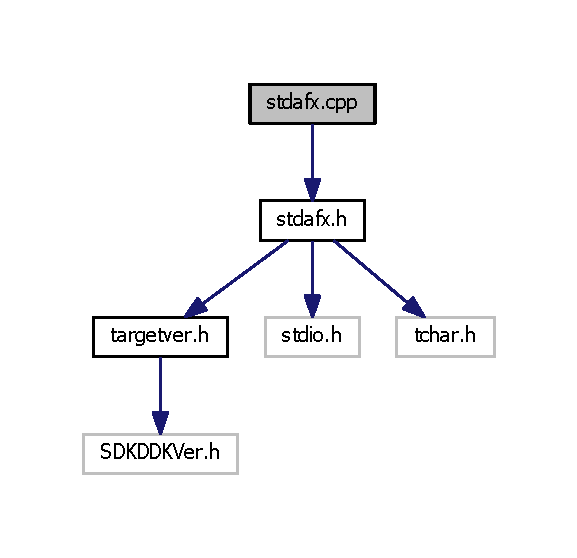
\includegraphics[width=277pt]{stdafx_8cpp__incl}
\end{center}
\end{figure}

\hypertarget{stdafx_8h}{\section{stdafx.\-h File Reference}
\label{stdafx_8h}\index{stdafx.\-h@{stdafx.\-h}}
}
{\ttfamily \#include \char`\"{}targetver.\-h\char`\"{}}\\*
{\ttfamily \#include $<$stdio.\-h$>$}\\*
{\ttfamily \#include $<$tchar.\-h$>$}\\*
Include dependency graph for stdafx.\-h\-:
\nopagebreak
\begin{figure}[H]
\begin{center}
\leavevmode
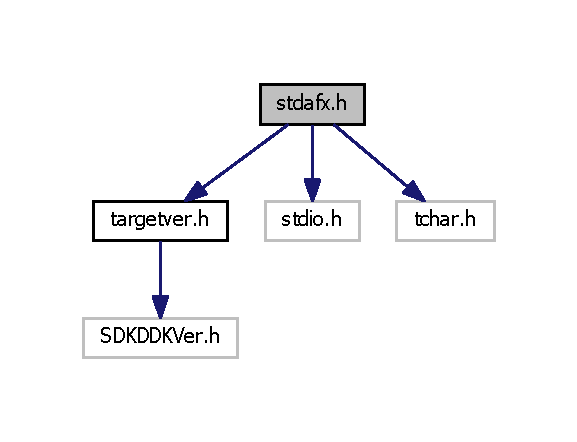
\includegraphics[width=277pt]{stdafx_8h__incl}
\end{center}
\end{figure}
This graph shows which files directly or indirectly include this file\-:
\nopagebreak
\begin{figure}[H]
\begin{center}
\leavevmode
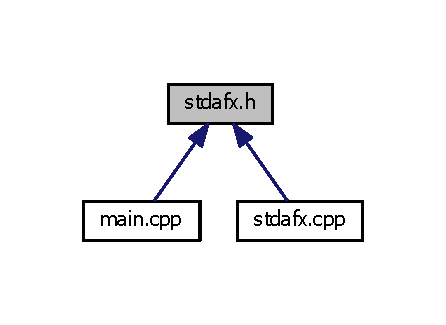
\includegraphics[width=214pt]{stdafx_8h__dep__incl}
\end{center}
\end{figure}

\hypertarget{targetver_8h}{\section{targetver.\-h File Reference}
\label{targetver_8h}\index{targetver.\-h@{targetver.\-h}}
}
{\ttfamily \#include $<$S\-D\-K\-D\-D\-K\-Ver.\-h$>$}\\*
Include dependency graph for targetver.\-h\-:
\nopagebreak
\begin{figure}[H]
\begin{center}
\leavevmode
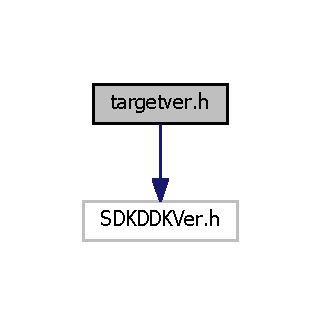
\includegraphics[width=154pt]{targetver_8h__incl}
\end{center}
\end{figure}
This graph shows which files directly or indirectly include this file\-:
\nopagebreak
\begin{figure}[H]
\begin{center}
\leavevmode
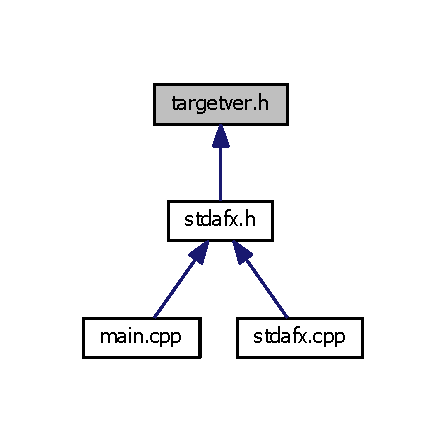
\includegraphics[width=214pt]{targetver_8h__dep__incl}
\end{center}
\end{figure}

%--- End generated contents ---

% Index
\newpage
\phantomsection
\addcontentsline{toc}{chapter}{Index}
\printindex

\end{document}
